\documentclass[a4paper,12pt]{article}
%%% Работа с русским языком % для pdfLatex
\usepackage{cmap}					% поиск в~PDF
\usepackage{mathtext} 				% русские буквы в~фомулах
\usepackage[T2A]{fontenc}			% кодировка
\usepackage[utf8]{inputenc}			% кодировка исходного текста
\usepackage[english,russian]{babel}	% локализация и переносы
\usepackage{indentfirst} 			% отступ 1 абзаца

%%% Работа с русским языком % для XeLatex
%\usepackage[english,russian]{babel}   %% загружает пакет многоязыковой вёрстки
%\usepackage{fontspec}      %% подготавливает загрузку шрифтов Open Type, True Type и др.
%\defaultfontfeatures{Ligatures={TeX},Renderer=Basic}  %% свойства шрифтов по умолчанию
%\setmainfont[Ligatures={TeX,Historic}]{Times New Roman} %% задаёт основной шрифт документа
%\setsansfont{Comic Sans MS}                    %% задаёт шрифт без засечек
%\setmonofont{Courier New}
%\usepackage{indentfirst}
%\frenchspacing

%%% Дополнительная работа с математикой
\usepackage{amsfonts,amssymb,amsthm,mathtools}
\usepackage{amsmath}
\usepackage{icomma} % "Умная" запятая: $0,2$ --- число, $0, 2$ --- перечисление
\usepackage{upgreek}

%% Номера формул
%\mathtoolsset{showonlyrefs=true} % Показывать номера только у тех формул, на которые есть \eqref{} в~тексте.

%%% Страница
\usepackage{extsizes} % Возможность сделать 14-й шрифт

%% Шрифты
\usepackage{euscript}	 % Шрифт Евклид
\usepackage{mathrsfs} % Красивый матшрифт

%% Свои команды
\DeclareMathOperator{\sgn}{\mathop{sgn}} % создание новой конанды \sgn (типо как \sin)
\usepackage{csquotes} % ещё одна штука для цитат
\newcommand{\pd}[2]{\ensuremath{\cfrac{\partial #1}{\partial #2}}} % частная производная
\newcommand{\abs}[1]{\ensuremath{\left|#1\right|}} % модуль
\renewcommand{\phi}{\ensuremath{\varphi}} % греческая фи
\newcommand{\pogk}[1]{\!\left(\cfrac{\sigma_{#1}}{#1}\right)^{\!\!\!2}\!} % для погрешностей

% Ссылки
\usepackage{color} % подключить пакет color
% выбрать цвета
\definecolor{BlueGreen}{RGB}{49,152,255}
\definecolor{Violet}{RGB}{120,80,120}
% назначить цвета при подключении hyperref
\usepackage[unicode, colorlinks, urlcolor=blue, linkcolor=blue, pagecolor=blue, citecolor=blue]{hyperref} %синие ссылки
%\usepackage[unicode, colorlinks, urlcolor=black, linkcolor=black, pagecolor=black, citecolor=black]{hyperref} % для печати (отключить верхний!)


%% Перенос знаков в~формулах (по Львовскому)
\newcommand*{\hm}[1]{#1\nobreak\discretionary{}
	{\hbox{$\mathsurround=0pt #1$}}{}}

%%% Работа с картинками
\usepackage{graphicx}  % Для вставки рисунков
\graphicspath{{images/}{images2/}}  % папки с картинками
\setlength\fboxsep{3pt} % Отступ рамки \fbox{} от рисунка
\setlength\fboxrule{1pt} % Толщина линий рамки \fbox{}
\usepackage{wrapfig} % Обтекание рисунков и таблиц текстом
\usepackage{multicol}

%%% Работа с таблицами
\usepackage{array,tabularx,tabulary,booktabs} % Дополнительная работа с таблицами
\usepackage{longtable}  % Длинные таблицы
\usepackage{multirow} % Слияние строк в~таблице
\usepackage{caption}
\captionsetup{labelsep=period, labelfont=bf}

%%% Оформление
\usepackage{indentfirst} % Красная строка
%\setlength{\parskip}{0.3cm} % отступы между абзацами
%%% Название разделов
\usepackage{titlesec}
\titlelabel{\thetitle.\quad}
\renewcommand{\figurename}{\textbf{Рис.}}		%Чтобы вместо figure под рисунками писал "рис"
\renewcommand{\tablename}{\textbf{Таблица}}		%Чтобы вместо table над таблицами писал Таблица

%%% Теоремы
\theoremstyle{plain} % Это стиль по умолчанию, его можно не переопределять.
\newtheorem{theorem}{Теорема}[section]
\newtheorem{proposition}[theorem]{Утверждение}

\theoremstyle{definition} % "Определение"
\newtheorem{definition}{Определение}[section]
\newtheorem{corollary}{Следствие}[theorem]
\newtheorem{problem}{Задача}[section]

\theoremstyle{remark} % "Примечание"
\newtheorem*{nonum}{Решение}
\newtheorem{zamech}{Замечание}[theorem]

%%% Правильные мат. символы для русского языка
\renewcommand{\epsilon}{\ensuremath{\varepsilon}}
\renewcommand{\phi}{\ensuremath{\varphi}}
\renewcommand{\kappa}{\ensuremath{\varkappa}}
\renewcommand{\le}{\ensuremath{\leqslant}}
\renewcommand{\leq}{\ensuremath{\leqslant}}
\renewcommand{\ge}{\ensuremath{\geqslant}}
\renewcommand{\geq}{\ensuremath{\geqslant}}
\renewcommand{\emptyset}{\varnothing}

\usepackage{bm} %жирный греческий шрифт
%\usepackage{ulem}

\graphicspath{{images}}

\title{Laba}
\author{Гадецкий Дмитрий}
\date{today}
\usepackage[left=1.27cm,right=1.27cm,top=2cm,bottom=2cm]{geometry}
\usepackage{bigstrut}
\usepackage{comment}
\usepackage{makecell}
\usepackage{float}

\begin{document}
\begin{titlepage}
\begin{center} 
 
\large Московский физико-технический институт\\
Факультет молекулярной и химической физики\\
\vspace{7cm}
\huge Лабораторная работа\\
\textbf{\Large <<ИЗМЕРЕНИЕ ВРАЩАТЕЛЬНОЙ И
	КОЛЕБАТЕЛЬНОЙ ТЕМПЕРАТУР
	В ГАЗОВОМ РАЗРЯДЕ
	ПО СПЕКТРУ МОЛЕКУЛЫ>>}\\
\end{center} 

\vspace{7.5cm}
{\par \raggedleft \large \emph{Выполнили:}\\ 
	студент 3 курса\\ 
	642 группы ФМХФ\\ 
	Гадецкий Дмитрий, \par
	студент 3 курса\\ 
	642 группы ФМХФ\\ 
	Маслак Никита \par
}
\begin{center}
\vfill \today
\date \today
\end{center}
\end{titlepage}
\newpage
%\setcounter{page}{2}
\renewcommand{\baselinestretch}{1.3}
\begin{center}
	\vspace{0.5cm}{\parbox{16cm}{\small{\centering{\textbf{Аннотация}\\
					\hspace{0.6cm} В этом отчёте изложены результаты выполнения лабораторной работы «».
				}}}}
\end{center}

\textbf{\emph{Цель работы:}} .
\section{Теоретическое введение}
\newpage
\section{Экспериментальная установка}
Принципиальная схема релаксометра ЯМР приведена на рис. \ref{fig:installation}

\begin{figure}[h]
	\centering
	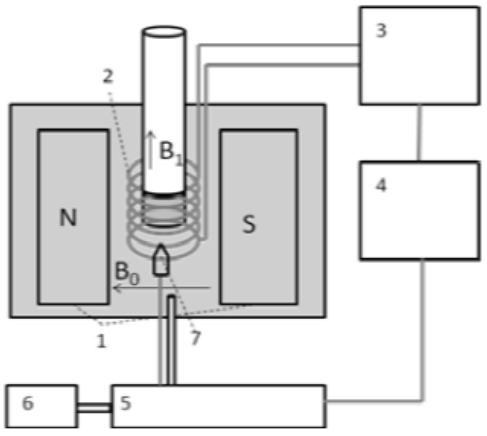
\includegraphics[width=0.6\linewidth]{Installation}
	\caption{Принципиальная схема: \textbf{1} -- постоянный магнит; \textbf{2} -- приемопередающая катушка; \textbf{3} -- генератор импульсов и приемник излучения; \textbf{4} -- компьютер; \textbf{5} -- система термостатирования образца; \textbf{6} -- воздушный компрессор; \textbf{7} -- термопара}
	\label{fig:installation}
\end{figure}

Основной частью ЯМР-релаксометра является магнит (\textbf{1} на рис. \ref{fig:installation}), создающий постоянное магнитное поле напряженностью $ \vec{B}_0 $. 

Переменное магнитное поле, перпендикулярное постоянному магнитному полю, создается при помощи катушки индуктивности, вдоль оси которой располагается пробирка с исследуемым образцом. Параллельно катушке включен конденсатор так, что образованный радиочастотный контур настроен на резонансную ларморовскую частоту.

Для созданя импульсов переменного поля катушка \textbf{2} соединяется с радиочастотным генератором, расположенным в \textbf{3}. Слабый сигнал ЯМР предварительно усиливается, затем поступает в блок управляющей электроники, где и производится его детектирование. При этом следует учитывать наличие переходных процессов в приемном контуре и усилителе, из-за которых у приемника существует т.н. <<мертвое время>> порядка 100 нс, необходимое для переключения в режим приема и усиления слабого сигнала намагниченности после периода генерации мощных импульсов.

\subsection{Ход работы}
\begin{enumerate}
	\item Получение результатов ЯМР в программе
	\item Изучение общего вида спектра при различных рабочих частотах
	\item Определение химического сдвига и относительной интенсивности составляющих спектра
	\item Исследование тонкой структуры, выводы и оценка неоднородности поля 
\end{enumerate}

\newpage
\section{Обработка результатов измерений}
Изобразим спектры при трех разных температурах: $40^\circ C,~ 55^\circ C,~ 70^\circ C$
\begin{figure}[H]%{r}{0.3\linewidth}
\centering
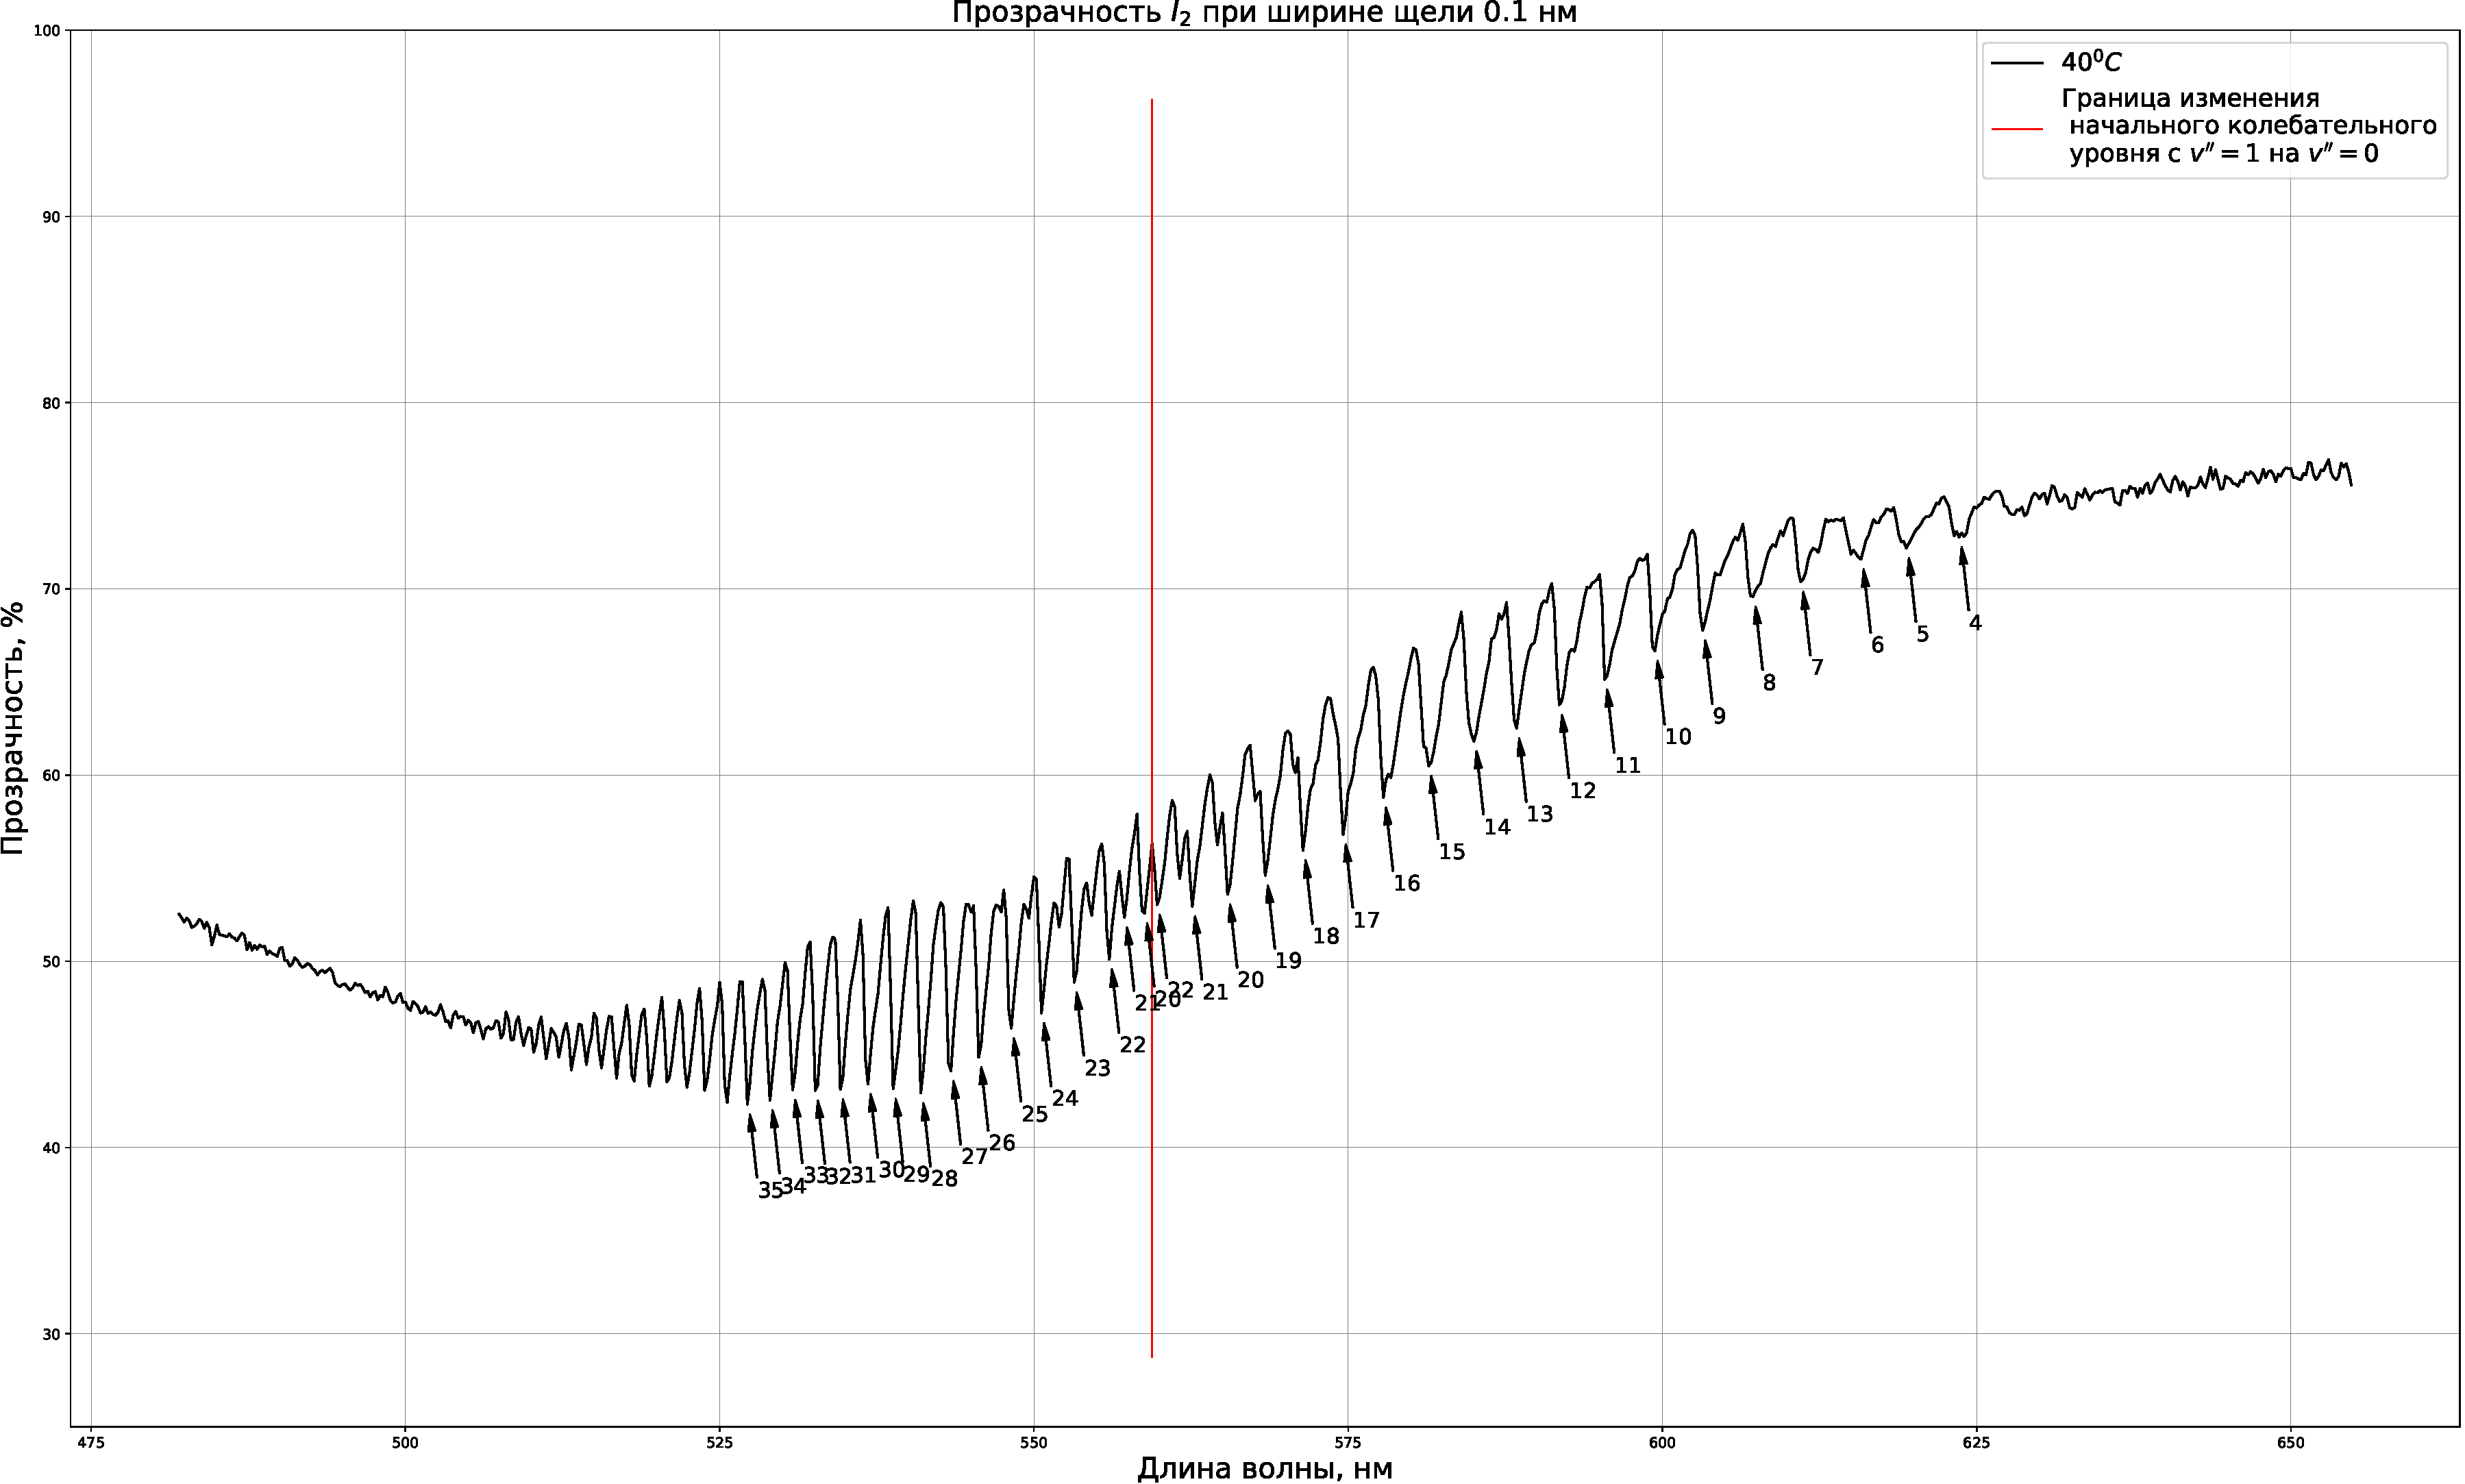
\includegraphics[angle = 90, height=0.87\textheight]{data/40_grad}
\caption{Спектр поглощения молекулы I$_2$, 40 $^\circ C$}
\label{40_graph}
\end{figure}
\begin{figure}[H]%{r}{0.3\linewidth}
\centering
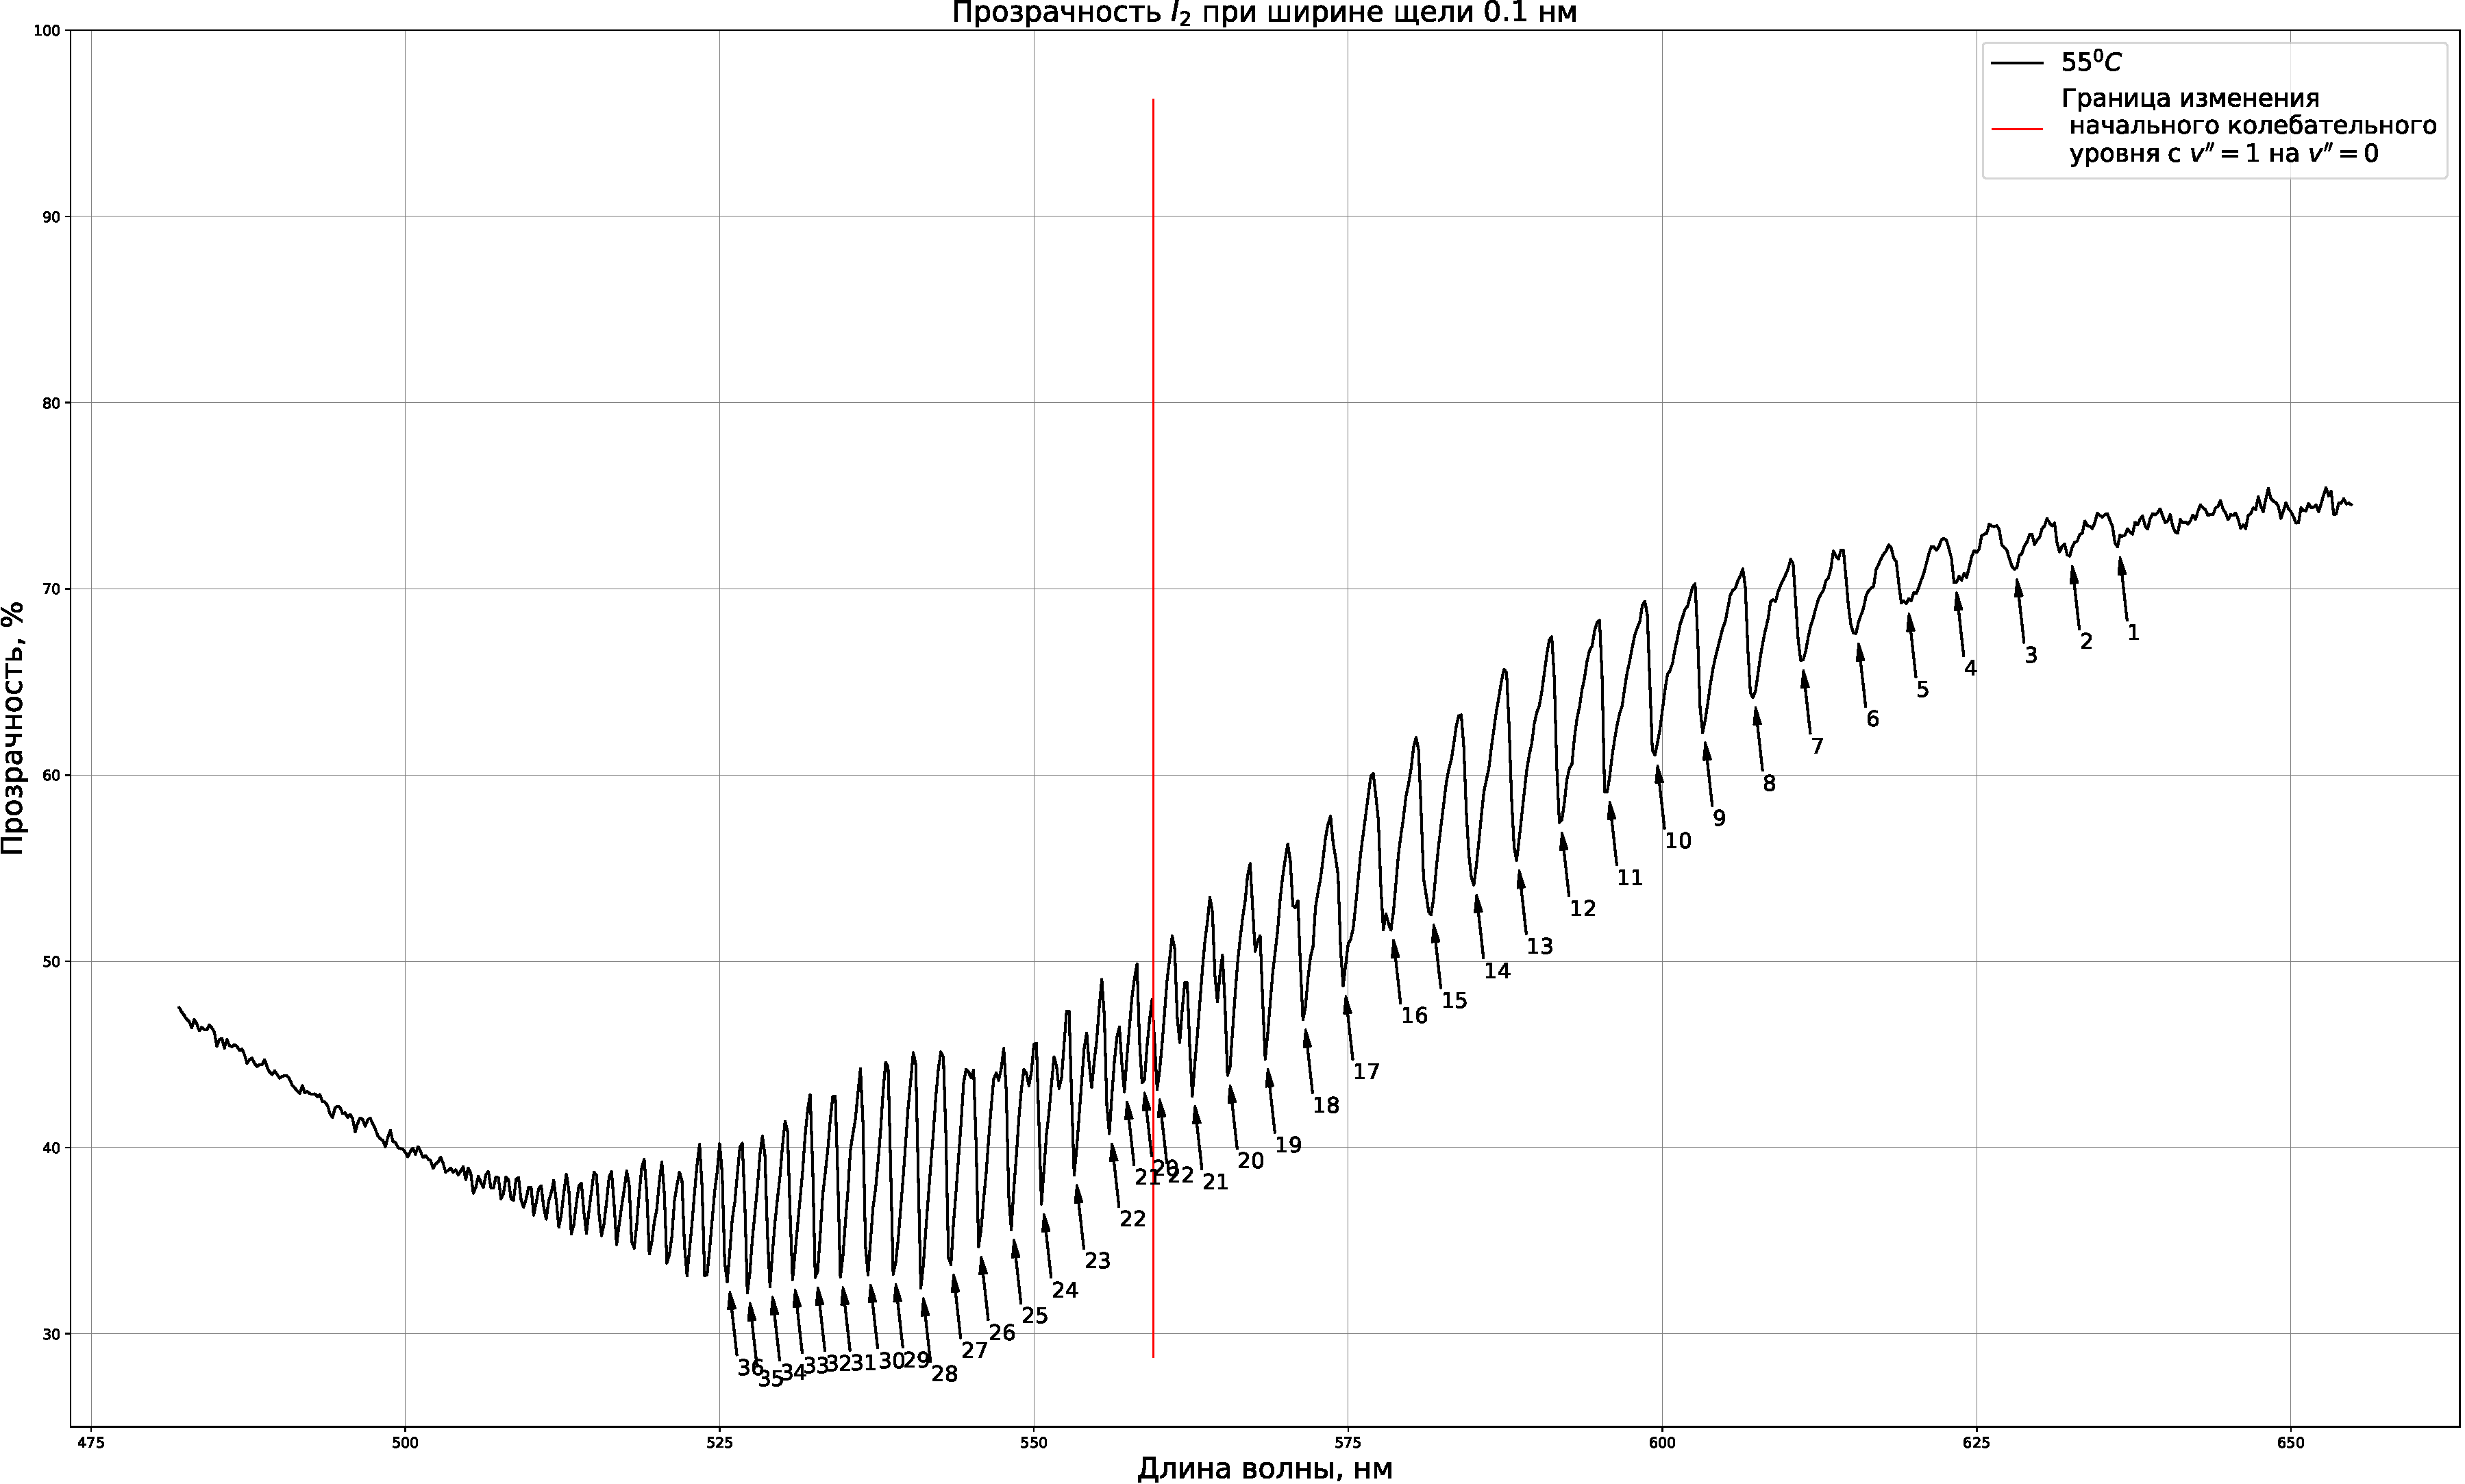
\includegraphics[angle = 90, height=0.95\textheight]{data/55_grad}
\caption{Спектр поглощения молекулы I$_2$, 55 $^\circ C$}
\label{55_graph}
\end{figure}
\begin{figure}[H]%{r}{0.3\linewidth}
\centering
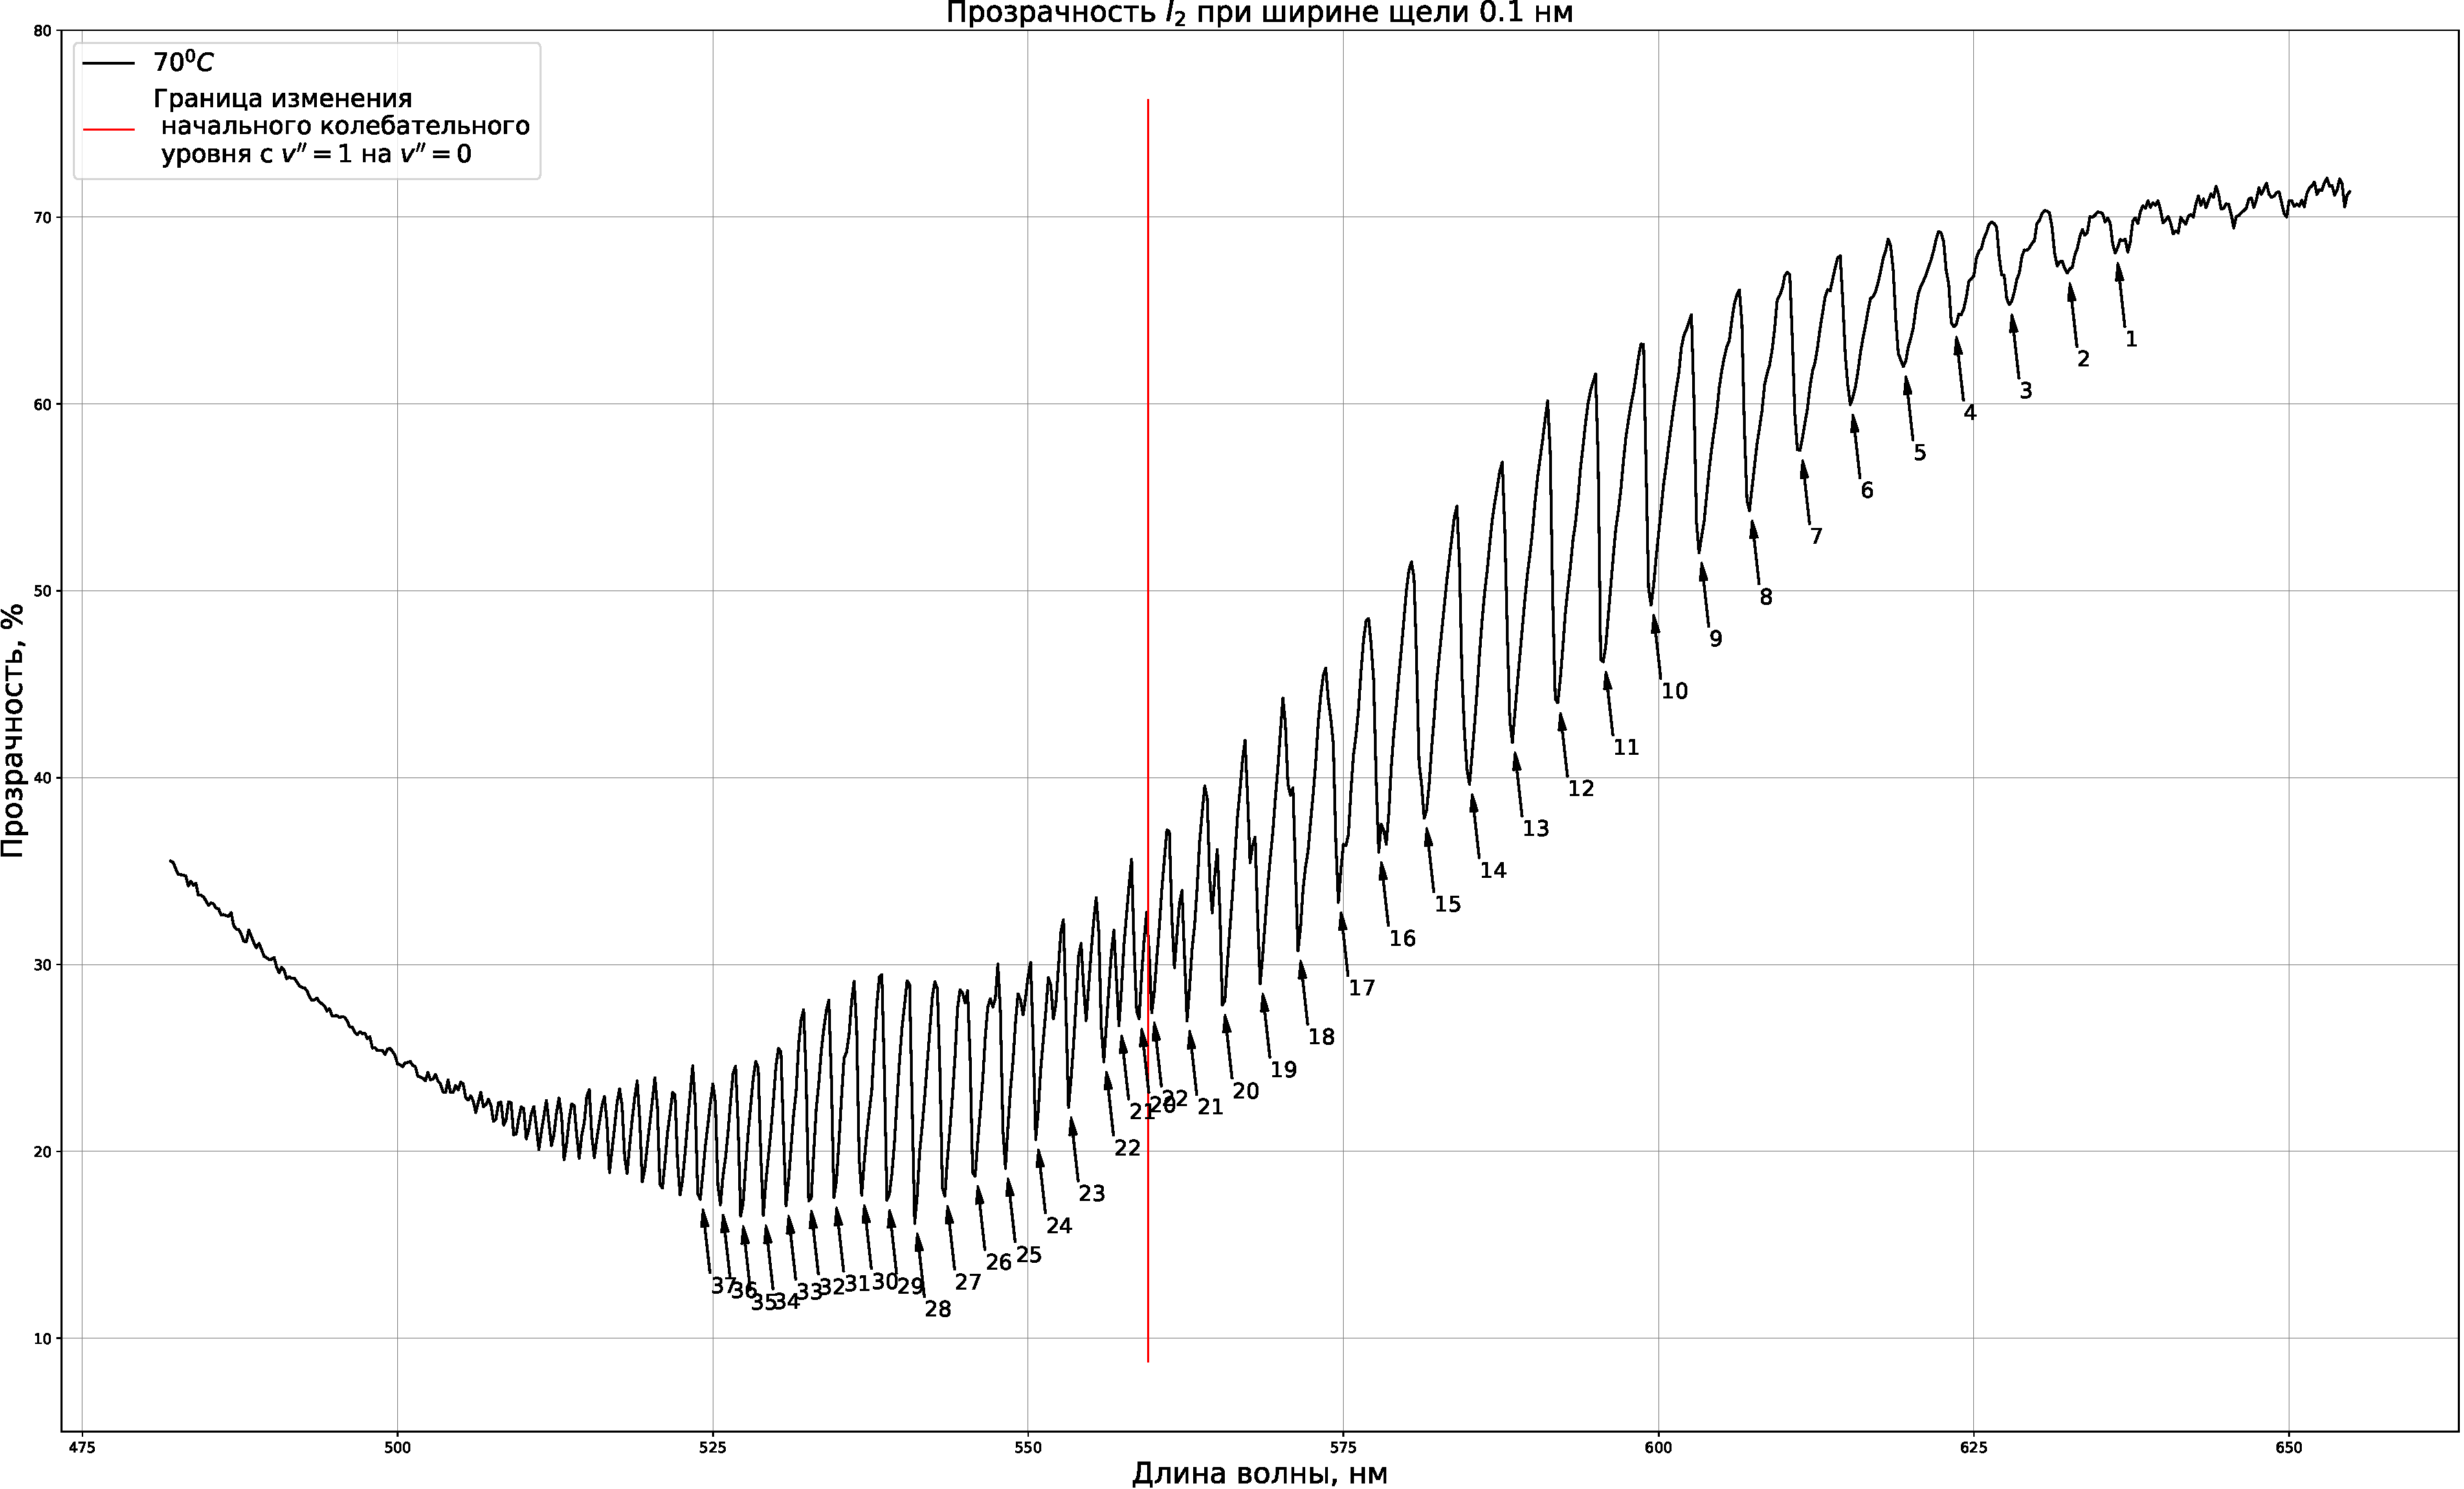
\includegraphics[angle = 90, height=0.95\textheight]{data/70_grad}
\caption{Спектр поглощения молекулы I$_2$, 70 $^\circ C$}
\label{70_graph}
\end{figure}

\newpage
\subsection{Построение таблицы Деландра и анализ спектра}
Изобразим спектры при трех разных температурах на рис. \ref{main_spectrum}.
\begin{figure}[h!]
	\centering
	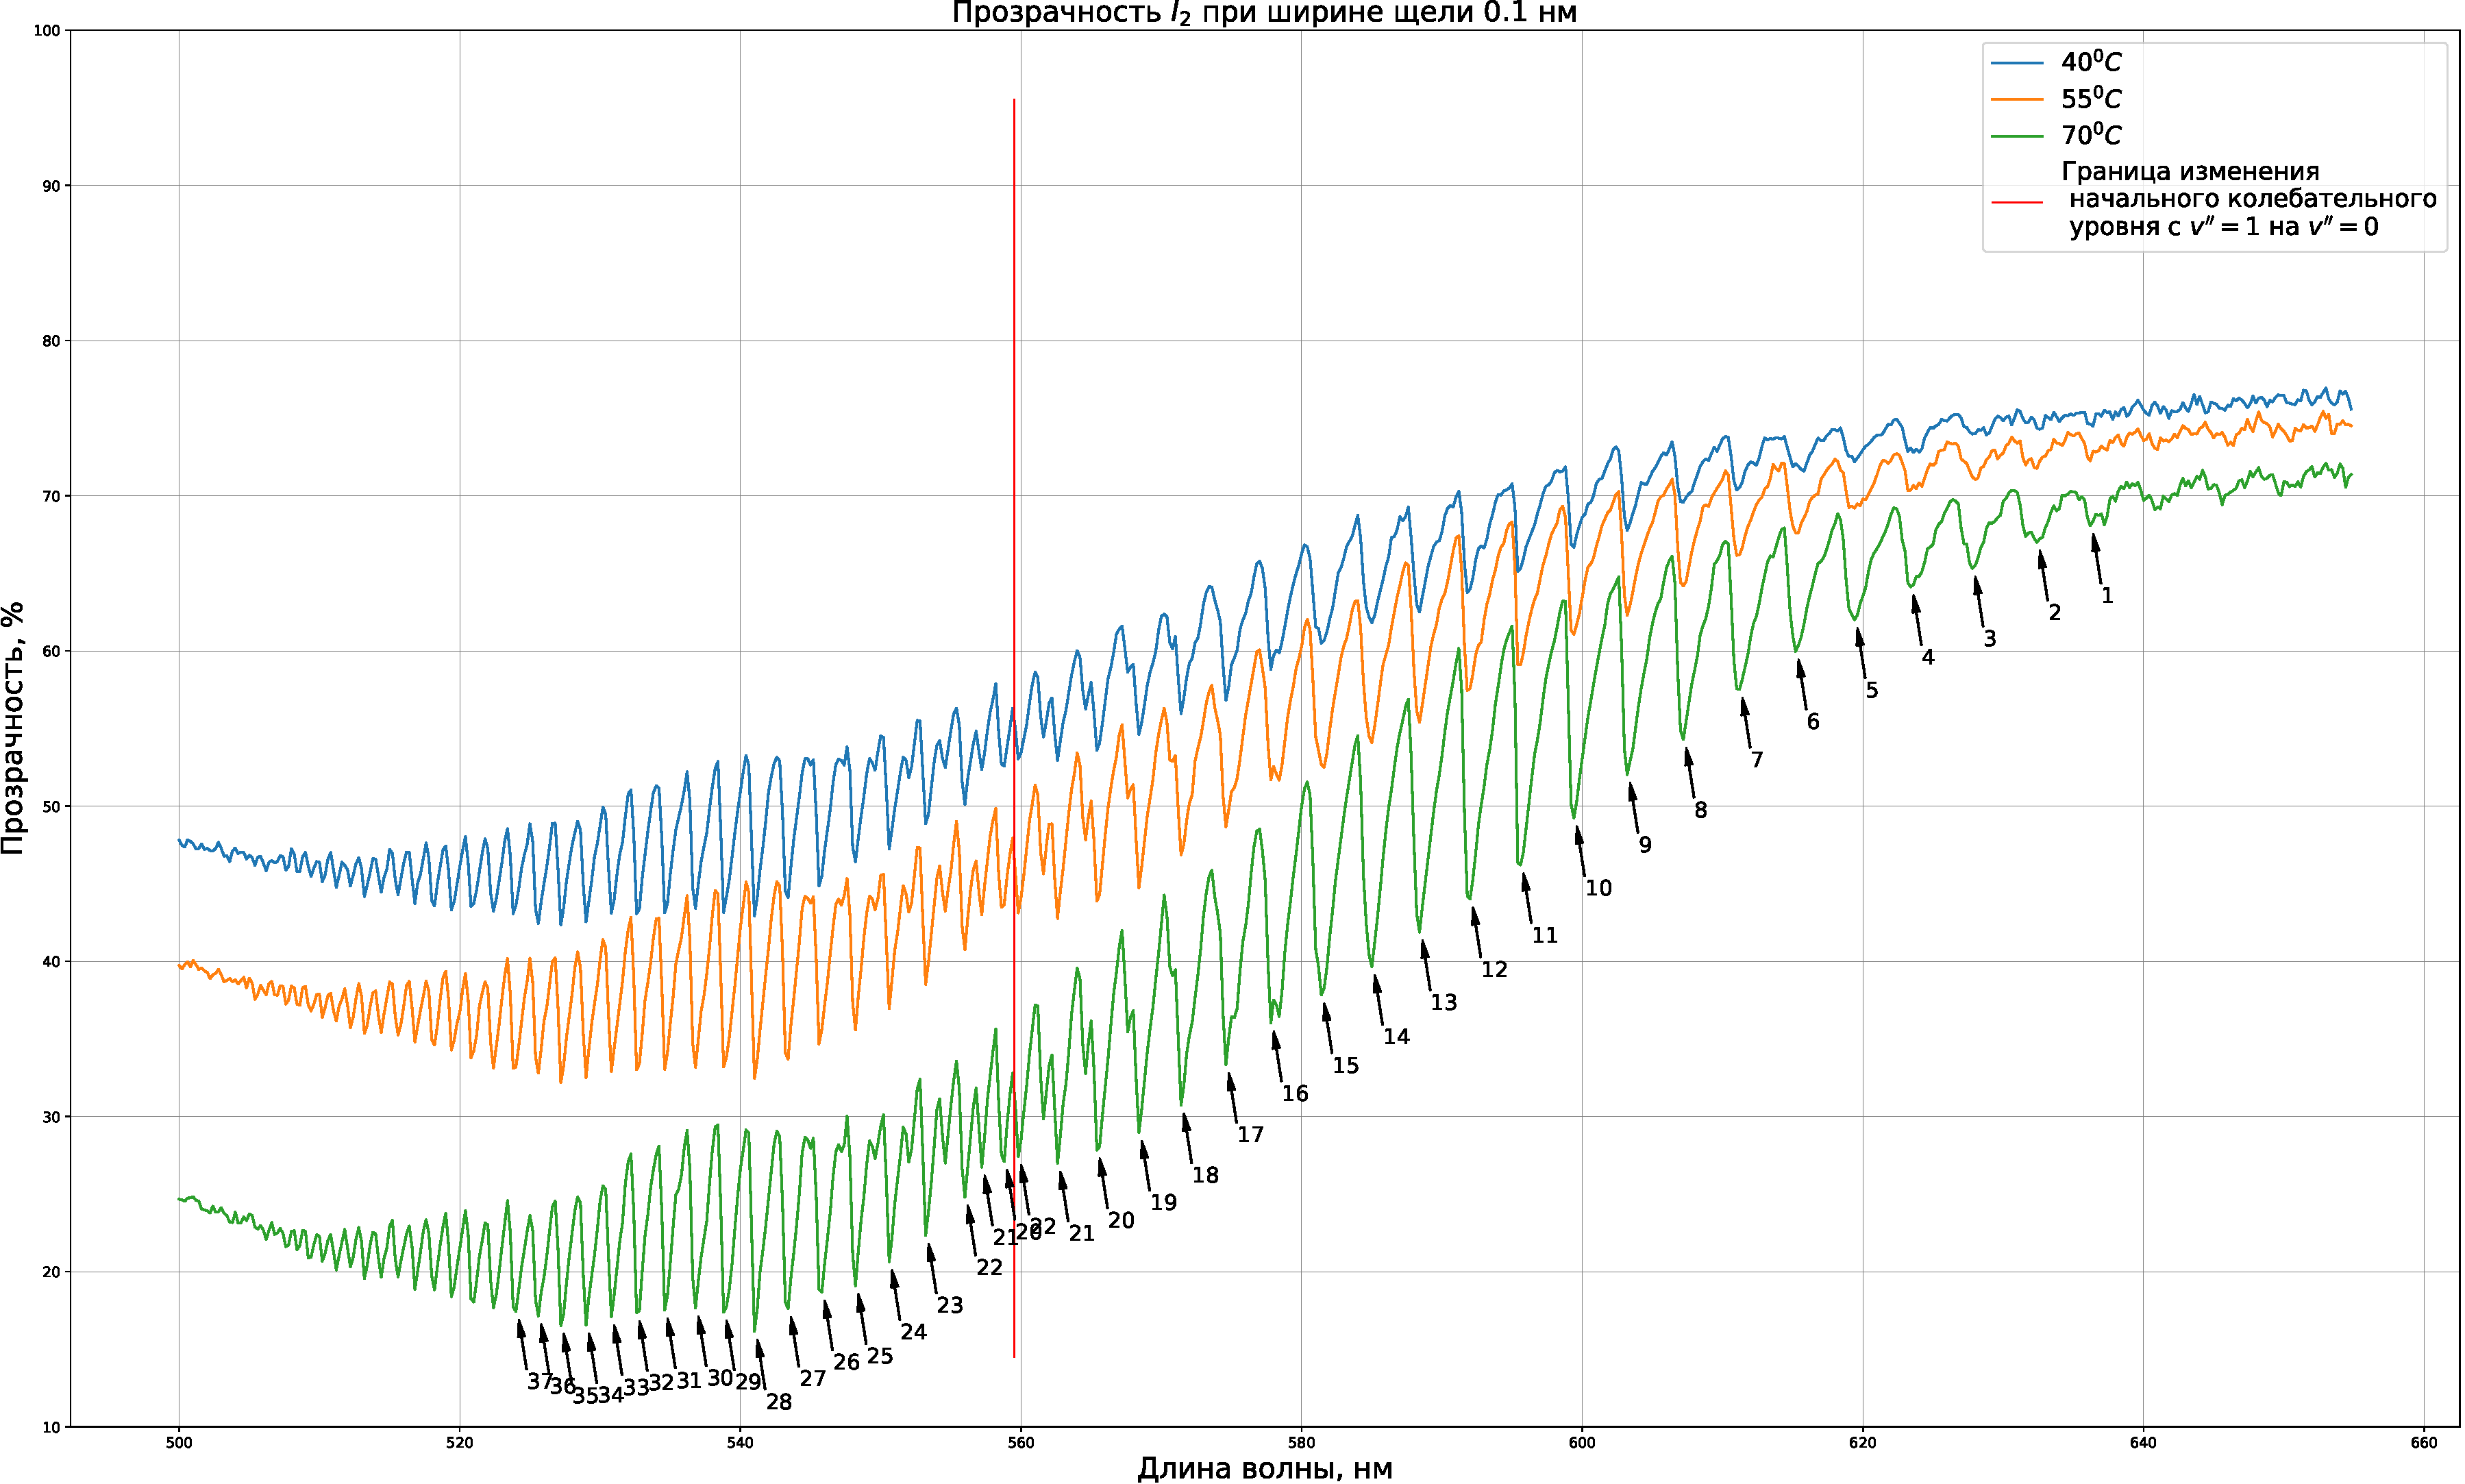
\includegraphics[angle = 90,
	% Высоту не менять! Подогнана)))
	height=0.88\textheight]{data/main_spectrum}
	\caption{Спектр поглощения молекулы I$_2$}
	\label{main_spectrum}
\end{figure}
\newpage
Видим, что при повышении температуры переходы становятся более отчетливыми, а прозрачность уменьшается. 

По спектру при температуре 70 $^\circ C$ составим таблицу \ref{tab:delandr} Деландра.

\begin{longtable}[h!]{|p{1cm}|p{3cm}|p{3cm}|}
	\caption{Таблица Деландра}\label{tab:delandr}\\
	\hline
	v'\textbackslash{}v'' & 0, см$^{-1}$ & 1, см $^{-1}$ \bigstrut\\
	\hline
	\endfirsthead
	\multicolumn{3}{p{8cm}}%
	{\tablename\ \thetable\ -- \textit{Продолжение с предыдущей страницы}} \\
	\hline
	v'\textbackslash{}v'' & 0, см$^{-1}$ & 1, см$^{-1}$ \bigstrut\\
	\hline
	\endhead
	\hline \multicolumn{3}{p{8cm}}{\textit{Продолжение на следующей странице}} \\
	\endfoot
	\hline
	\endlastfoot
	\hline
	1 &   & 15718 \bigstrut\\
	\hline
	2 &   & 15812 \bigstrut\\
	\hline
	3 &   & 15928 \bigstrut\\
	\hline
	4 &   & 16041 \bigstrut\\
	\hline
	5 &   & 16144 \bigstrut\\
	\hline
	6 &   & 16254 \bigstrut\\
	\hline
	7 &   & 16361 \bigstrut\\
	\hline
	8 &   & 16469 \bigstrut\\
	\hline
	9 &   & 16578 \bigstrut\\
	\hline
	10 &   & 16683 \bigstrut\\
	\hline
	11 &   & 16789 \bigstrut\\
	\hline
	12 &   & 16891 \bigstrut\\
	\hline
	13 &   & 16995 \bigstrut\\
	\hline
	14 &   & 17094 \bigstrut\\
	\hline
	15 &   & 17199 \bigstrut\\
	\hline
	16 &   & 17307 \bigstrut\\
	\hline
	17 &   & 17403 \bigstrut\\
	\hline
	18 &   & 17500 \bigstrut\\
	\hline
	19 &   & 17593 \bigstrut\\
	\hline
	20 & 17889 & 17686 \bigstrut\\
	\hline
	21 & 17985 & 17774 \bigstrut\\
	\hline
	22 & 18076 & 17863 \bigstrut\\
	\hline
	23 & 18162 &  \bigstrut\\
	\hline
	24 & 18241 &  \bigstrut\\
	\hline
	25 & 18321 &  \bigstrut\\
	\hline
	26 & 18402 &  \bigstrut\\
	\hline
	27 & 18484 &  \bigstrut\\
	\hline
	28 & 18559 &  \bigstrut\\
	\hline
	29 & 18628 &  \bigstrut\\
	\hline
	30 & 18705 &  \bigstrut\\
	\hline
	31 & 18775 &  \bigstrut\\
	\hline
	32 & 18839 &  \bigstrut\\
	\hline
	33 & 18903 &  \bigstrut\\
	\hline
	34 & 18968 &  \bigstrut\\
	\hline
	35 & 19025 &  \bigstrut\\
	\hline
	36 & 19083 &  \bigstrut\\
	\hline
\end{longtable}
\subsection{Линейная аппроксимация}
Вычислим разности соседних волновых чисел в полученных $v'$-прогрессиях \\$\nu(v'+1)-\nu(v')= \Delta G'_{v'+0.5}$. Используя полученные значения, проведем регрессионный анализ зависимости $\Delta G'_{v'+0.5}(v'+1)$ при $v'' = 0; 1$ (рис. \ref{deltaG0}, \ref{deltaG1}).

\begin{figure}[h!]
	\centering
	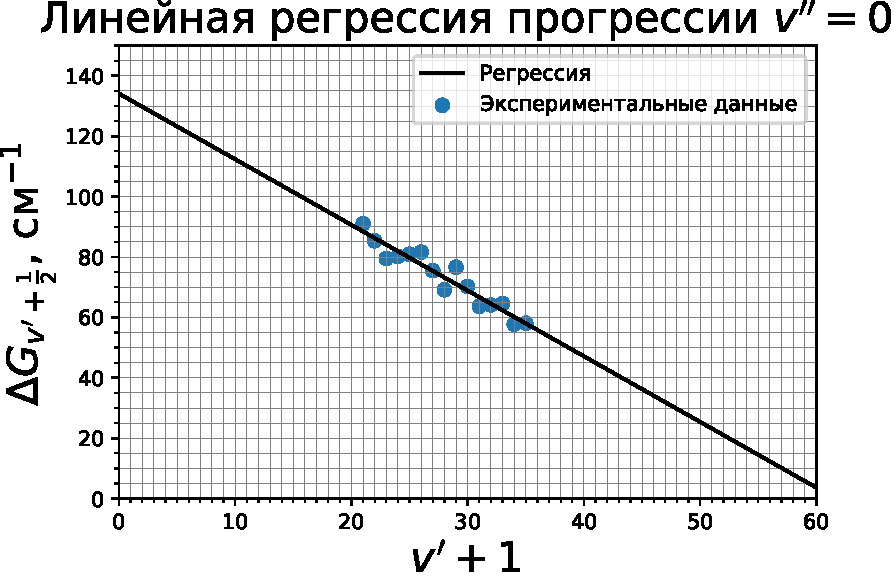
\includegraphics[width=0.81\linewidth]{data/deltaG(v_0).pdf}
	\caption{Линейная аппроксимация ($v''=0$)}
	\label{deltaG0}
\end{figure}
\begin{figure}[h!]
	\centering
	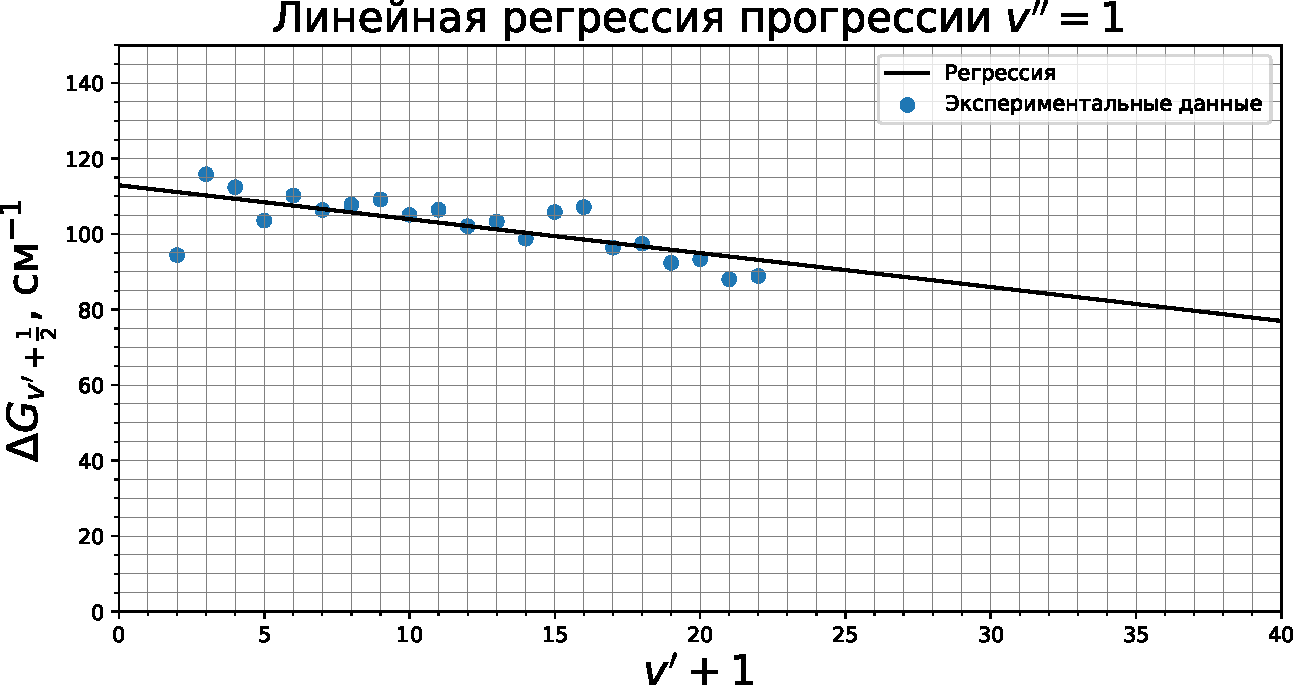
\includegraphics[width=0.79\linewidth]{data/deltaG(v_1).pdf}
	\caption{Линейная аппроксимация ($v''=1$)}
	\label{deltaG1}
\end{figure}

Отсюда, получаем результат (табл. \ref{tab:linear_approx}).
% Table generated by Excel2LaTeX from sheet 'Пункт 3'
\begin{table}[h!]
	\centering
	\caption{Результаты линейной аппроксимации}
	\begin{tabular}{|c|c|c|c|}
		\hline
		\multicolumn{1}{|l|}{v''} & \multicolumn{1}{l|}{$\omega_e'$, см$^{-1}$} & \multicolumn{1}{l|}{$\omega_e' x_e'$, см$^{-1}$} & \multicolumn{1}{c|}{$\rho$} \bigstrut\\
		\hline
		0 & $134\pm 3$ & $1.09\pm 0.05$& -0.96 \bigstrut\\
		\hline
		1 & $113\pm 3$& $0.45\pm 0.13$ & -0.72 \bigstrut\\
		\hline
	\end{tabular}%
	\label{tab:linear_approx}%
\end{table}%

\subsection{Определение молекулярных констант методом параболического регрессионного анализа}

Определим значение $\omega'_e$, $\omega'_e x_e'$, а также величину электронного терма $T_e$ возбужденного состояния $^3\Pi^+_{0u}$, используя зависимость \eqref{wave_counts}:
\begin{equation}
\nu = \nu_{\text{эл}} + \left[\omega'_e\left(v'+\frac{1}{2}\right)-\omega'_e x_e'\left(v'+\frac{1}{2}\right)^2\right]-\left[\omega''_e\left(v''+\frac{1}{2}\right)-\omega''_e x_e''\left(v''+\frac{1}{2}\right)^2\right].
\label{wave_counts}
\end{equation}
Применяя метод параболического регрессионного анализа для выделенных $v'$ прогрессий, получим рис. \ref{parabola_half_0}, \ref{parabola_half_1}, а численный результат занесем в таблицу \ref{tab:parabola}.
\begin{figure}[h!]
	\centering
	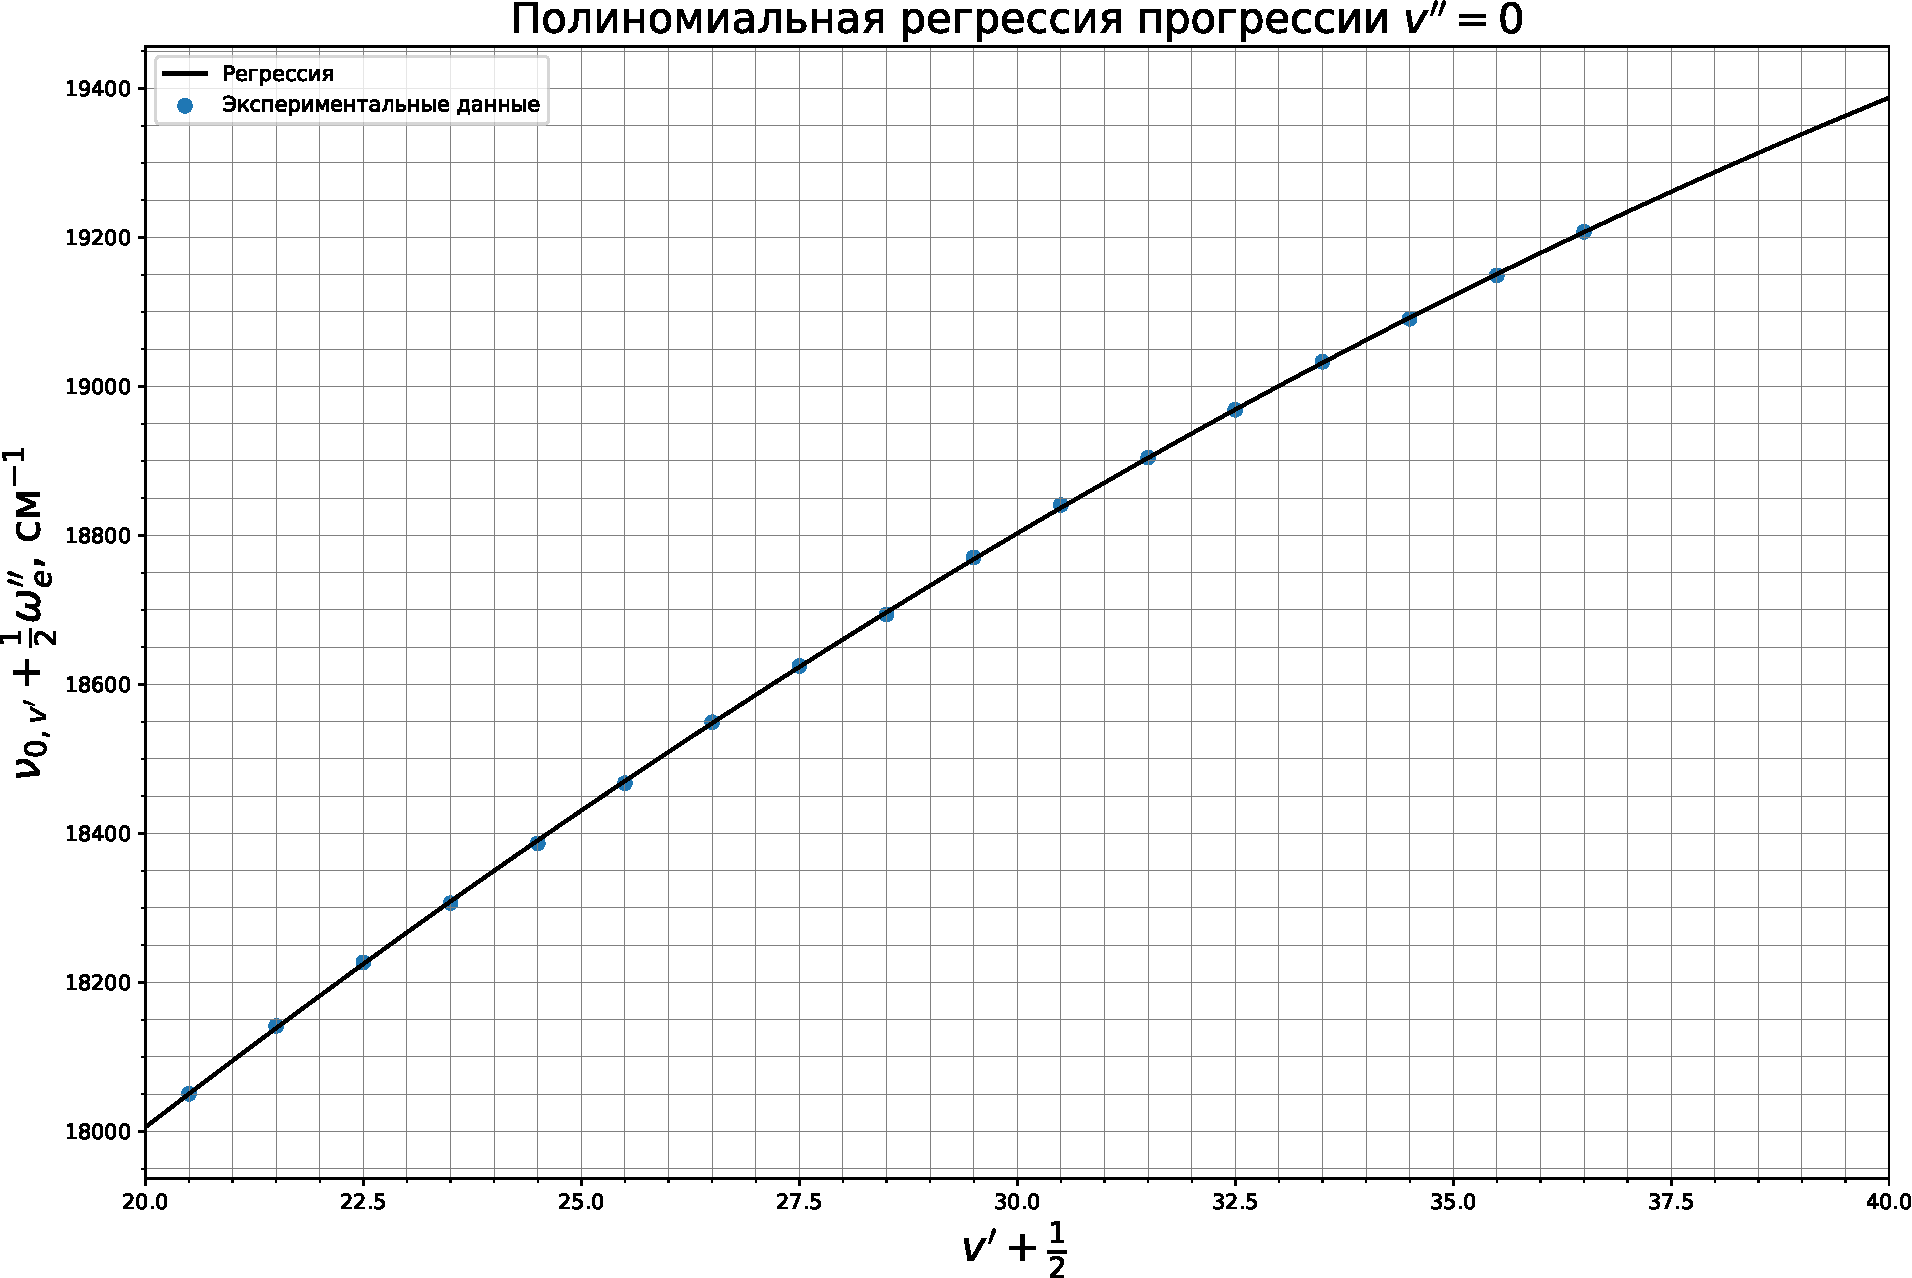
\includegraphics[height=0.4\textheight]{data/parabola_half_0}
	\caption{Параболическая аппроксимация ($v'' = 0$)}
	\label{parabola_half_0}
\end{figure}
\begin{figure}[h!]
	\centering
	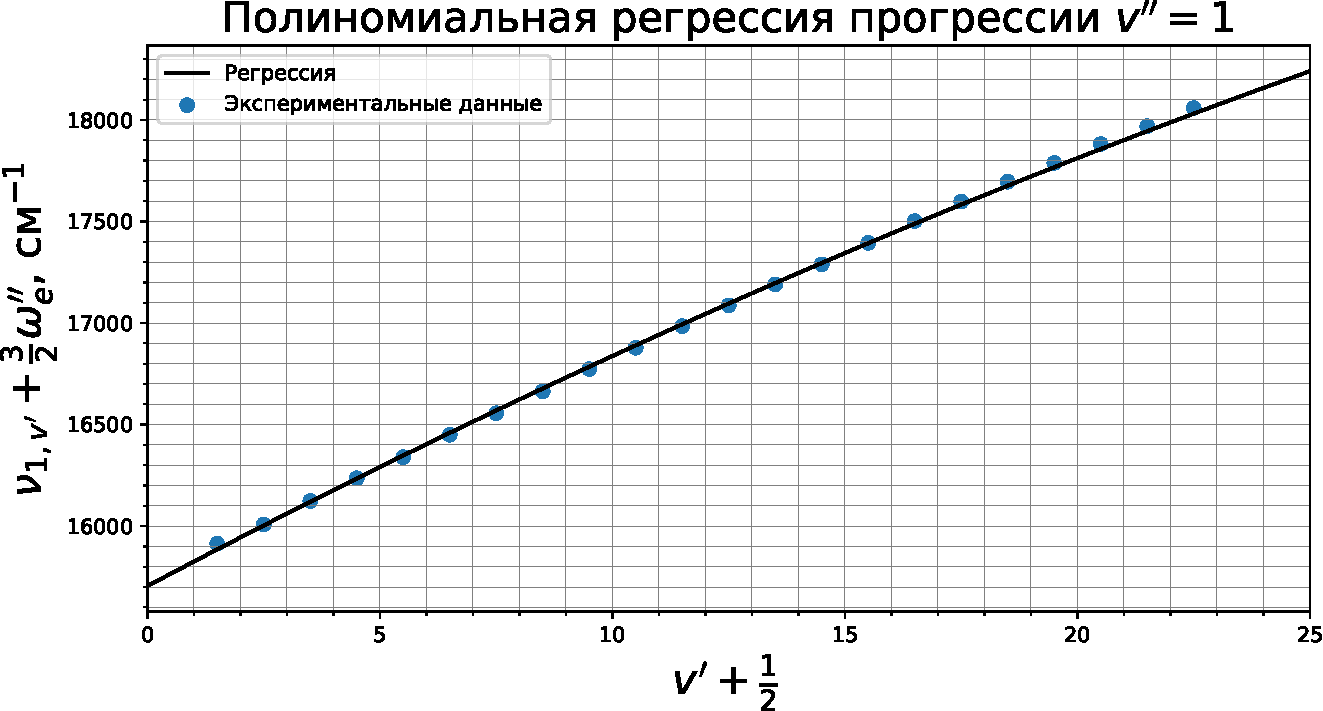
\includegraphics[height=0.4\textheight]{data/parabola_half_1}
	\caption{Параболическая аппроксимация ($v'' = 1$)}
	\label{parabola_half_1}
\end{figure}

% Table generated by Excel2LaTeX from sheet '4 пункт'
\begin{table}[htbp]
	\centering
	\caption{Результаты анализа для выделенных $v'$ прогрессий}
	\begin{tabular}{|r|r|r|r|}
		\hline
		\multicolumn{1}{|l|}{v''} & \multicolumn{1}{l|}{$T_e$, см$^{-1}$} & \multicolumn{1}{l|}{$\omega'_e$, см$^{-1}$} & \multicolumn{1}{l|}{$\omega'_e x'_e$, см$^{-1}$} \bigstrut\\
		\hline
		0 & 15774 & 132.8 & 1.06 \bigstrut\\
		\hline
		1 & 15705 & 121.1 & 0.78 \bigstrut\\
		\hline
	\end{tabular}%
	\label{tab:parabola}%
\end{table}%

Вычислим волновое число $\nu_{0,0} \cong T_e + 0.5\omega_e' - 0.5\omega_e''$ ($\omega_e''$ для $I_2$ равна $214$ см$^{-1}$)
\begin{equation}
\nu_{0,0} = 15750 \text{ см$^{-1}$}
\end{equation}


\subsection{Вычисление $\nu_{\text{гр}}$}
По экспериментальным значениям волновых чисел $\nu_{0,v'}$ для переходов $v''= 0 \to v'$ определим волновое число границы непрерывного спектра поглощения $\nu_{\text{гр}}$ , считая, что волновые числа полос $\nu(v')$ и их разности $\Delta \nu =\nu(v'+1)-\nu(v')$ связаны квадратичной зависимостью
вида \eqref{delta_nu}.
\begin{equation}
\nu = \nu_{\text{гр}} +b\Delta\nu+c\left(\Delta \nu\right)^2
\label{delta_nu}
\end{equation}
Результат аппроксимации параболой представлен на рис. \ref{fig:delta_nu}, а численное значение $\nu_{\text{гр}}$ есть
\begin{equation}
\nu_{\text{гр}} = (20.0 \pm 0.6) \cdot 10^3 \text{ см$^{-1}$}
\end{equation}
\begin{figure}[h!]
	\centering
	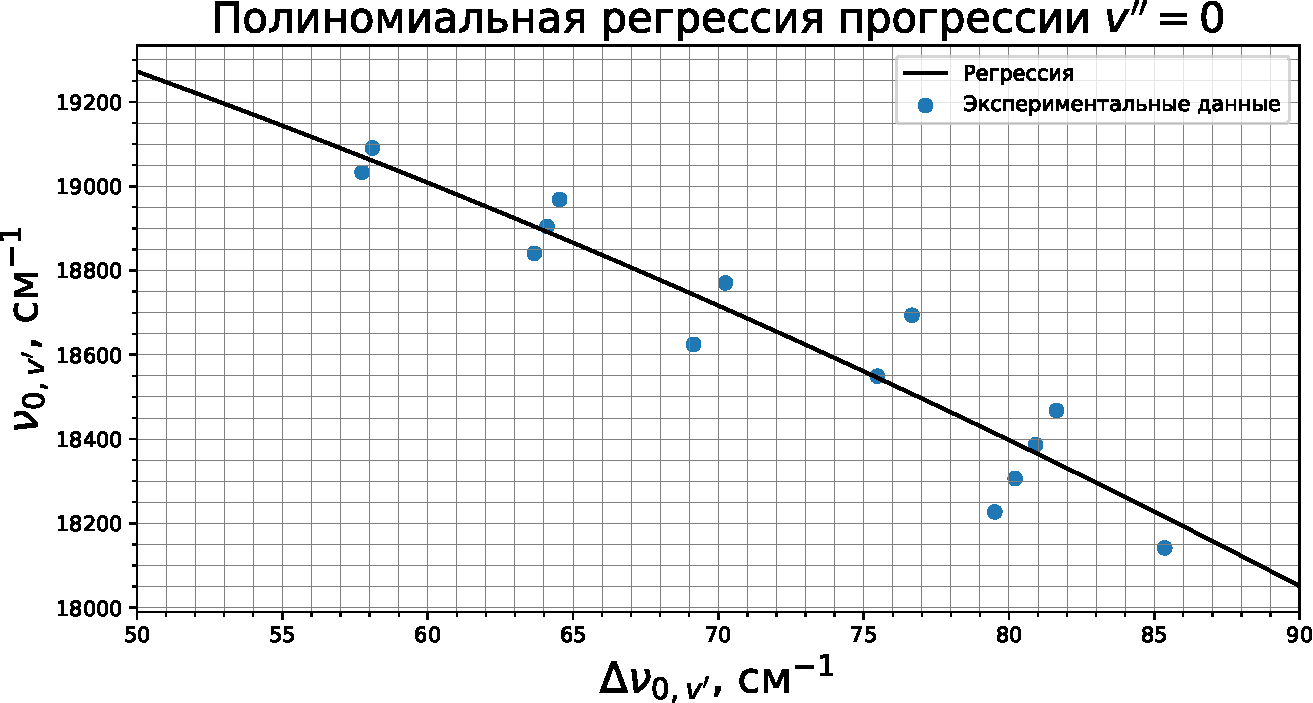
\includegraphics[height=0.35\textheight]{data/delta_nu}
	\caption{Определение границы сплошного спектра}
	\label{fig:delta_nu}
\end{figure}

\subsection{Определение энергий диссоциации}
Используя полученные ранее значения молекулярных постоянных, определим энергию диссоциации $D_0'$ для возбужденного электронного состояния $^3\Pi^+_{0u}$ тремя способами:
\begin{enumerate}
	\item По формуле линейной экстраполяции 
	\begin{equation}
	D_0'=\cfrac{\omega_e'^2}{4\omega_e'x_e'} = 4029 \text{ см$^{-1}$}
	\end{equation}
	\item По границе сплошного спектра
	\begin{equation}
	D_0'=\nu_{\text{гр}}- \nu_{00} = 4250 \text{ см$^{-1}$}
	\end{equation}
	\item Методом Берджа-Шпонер
\end{enumerate}
Для подсчета методом Берджа-Шпонер необходимо величины разностей $\Delta G'_{v'+0.5}$ отнести к серединам колебательных интервалов, т.е. к $v'+0.5$, а далее экстраполировать параболой (рис. \ref{fig:deltaG_half_berdg}). Площадь под этой кривой соответствует энергии диссоциации.
\begin{figure}[h!]
	\centering
	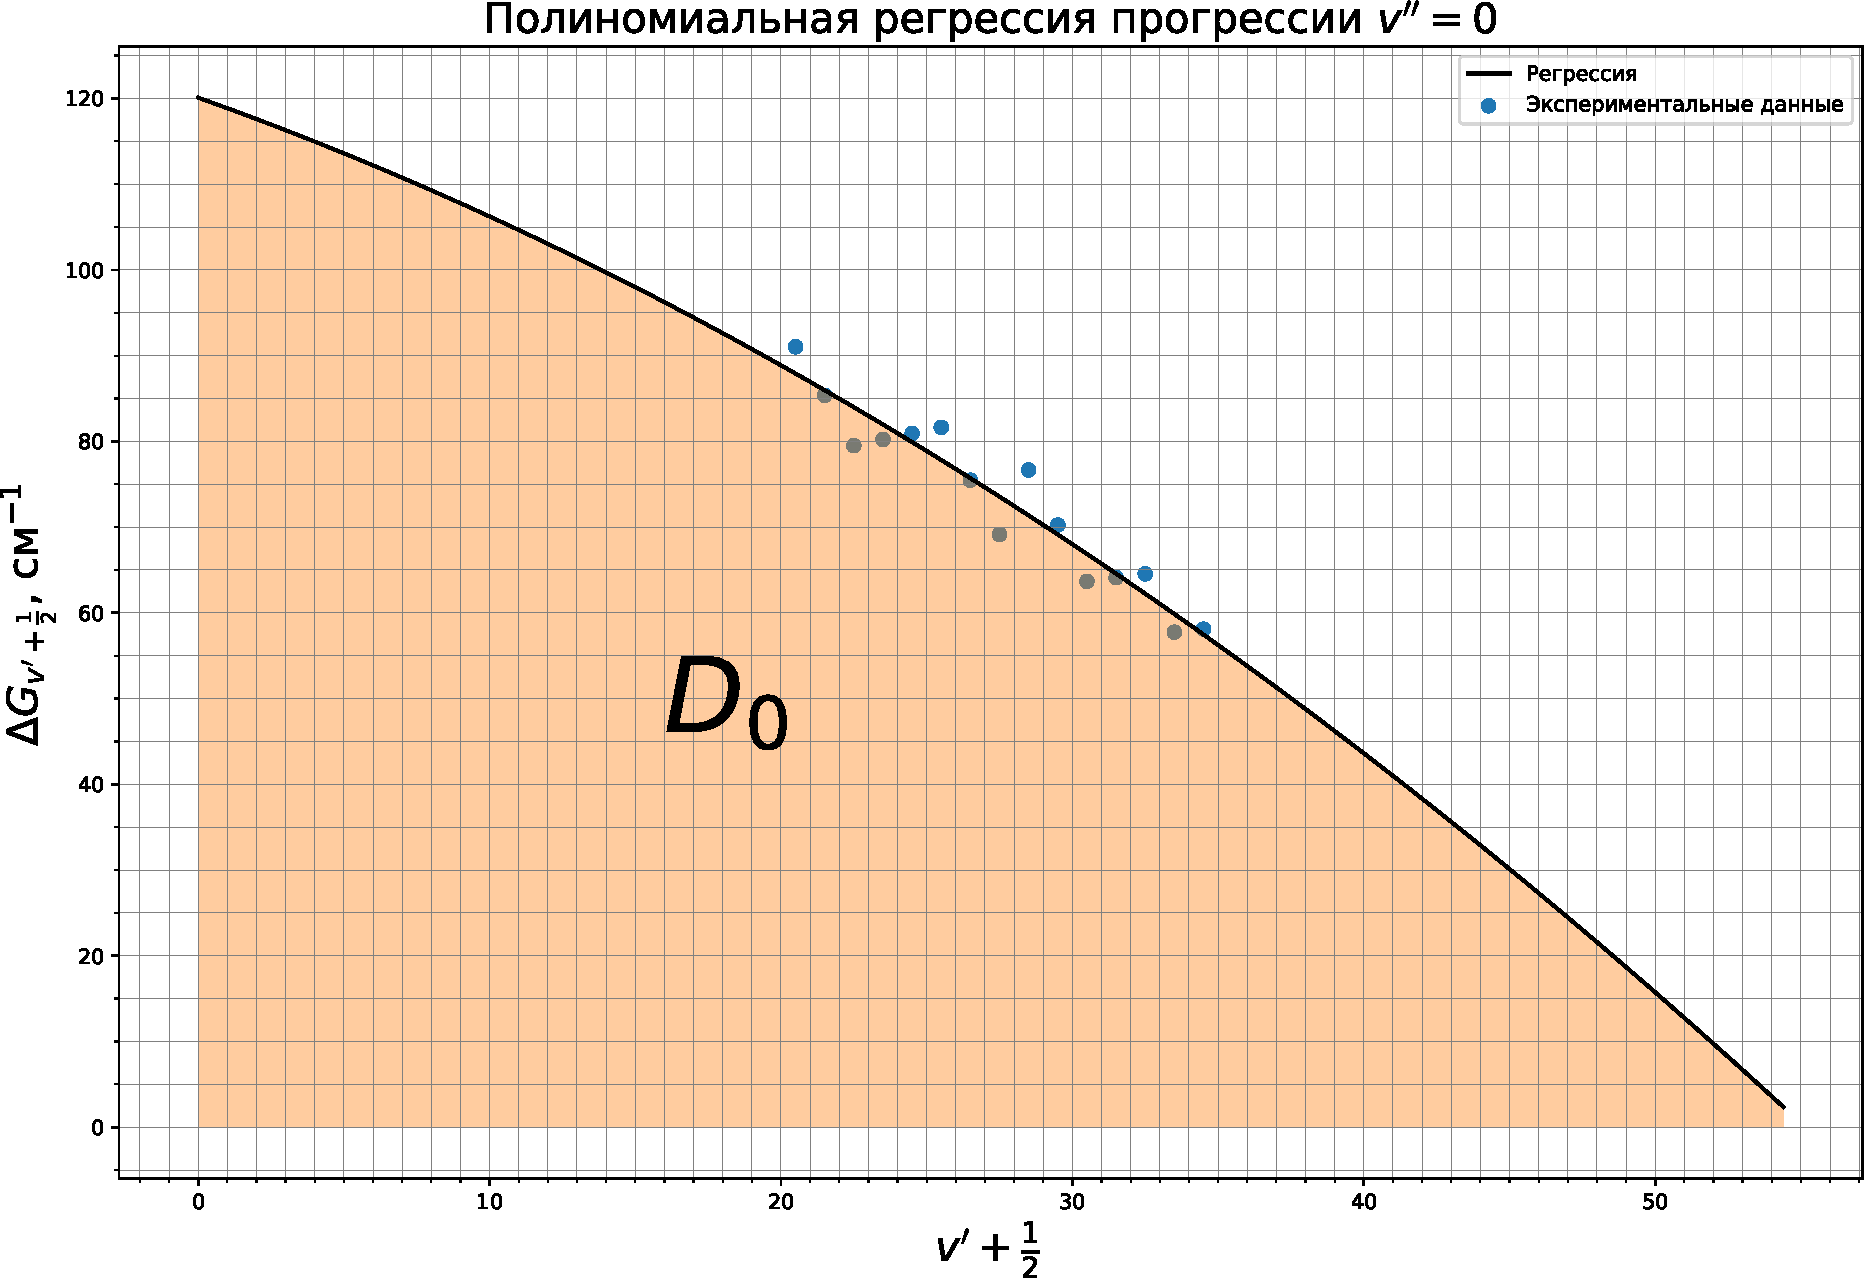
\includegraphics[height=0.45\textheight]{data/deltaG_half_berdg}
	\caption{Экстраполяция методом Берджа-Шпонер}
	\label{fig:deltaG_half_berdg}
\end{figure}
Проинтегрировав аппроксимацию, получим
\begin{equation}
D_0' = 3776 \text{ см$^{-1}$}
\end{equation}

Определим энергию диссоциации $D_0''$ для основного электронного состояния $^1\Sigma_g^{+}$ по границе сплошного спектра ($E_a = 7603$ см$^{-1}$)
\begin{equation}
D_0'' = \nu_{\text{гр}}-E_a = 12397 \text{ см$^{-1}$}
\end{equation}
\subsection{Определение межъядерного расстояния, построение потенциальной кривой Морзе}
Для прогрессии с $v'' = 0$ определим волновое число полосы с максимальным поглощением (у нас это пик под номером $28$)
\begin{equation}
\nu_{max}  = 18559 \text{ см$^{-1}$}
\end{equation}
Определим равновесное межъядерное положение $r_e'$ для возбужденного электронного состояния $^3\Pi^+_{0u}$, используя уравнения \eqref{eq:pot_en_r_e}, \eqref{eq:r_e'} и полученные из опыта значения $\nu_{max}, \omega_e', D_0'$. Примем, что $r_e'' = 2.67$ \AA.
\begin{equation}
\label{eq:pot_en_r_e}
U'(r'=r_e'') \cong \nu_{max} - \nu_{0,0}+\cfrac{\omega_e'}{2} = 3209 \text{ см}^{-1}
\end{equation}
\begin{equation}
\label{eq:r_e'}
r_e'=r_e'' + \frac{1}{\beta'}\,\ln\left[1+\left(\cfrac{U'(r'=r_e'')}{D_e'}\right)^{1/2}\right]
\end{equation}
где $D'_e \cong D'_0 + \dfrac{\omega'_e}{2} = 3839 \text{ см}^{-1},~ 
\beta' = \omega'_e \left( \dfrac{2 \pi^2 \mu c}{D'_e h} \right)^{1/2} 
\approx 0.122 \omega'_e \sqrt{ \dfrac{\mu}{D'_e} }
\approx 4.16 \text{ см}^{-1}$, если $\omega'_e$, $D'_e$ выражены в см$^{-1}$, $\mu$ - в а.е.м.

После численных подстановок получим
\begin{equation}
r_e' = 2.826 \text{ \AA}
\end{equation}
Построим потенциальную кривую возбужденного электронного состояния $^3\Pi^+_{0u}$, используя функцию Морзе (рис. \ref{fig:morse}). Для этого найдем $D'_e = D'_0 + hc(\frac{1}{2}\omega'_e - \frac{1}{4}\omega'_e x'_e) = 4215 \text{см}^{-1} = 0.527 \text{эВ}$
\begin{figure}[h!]
	\centering
	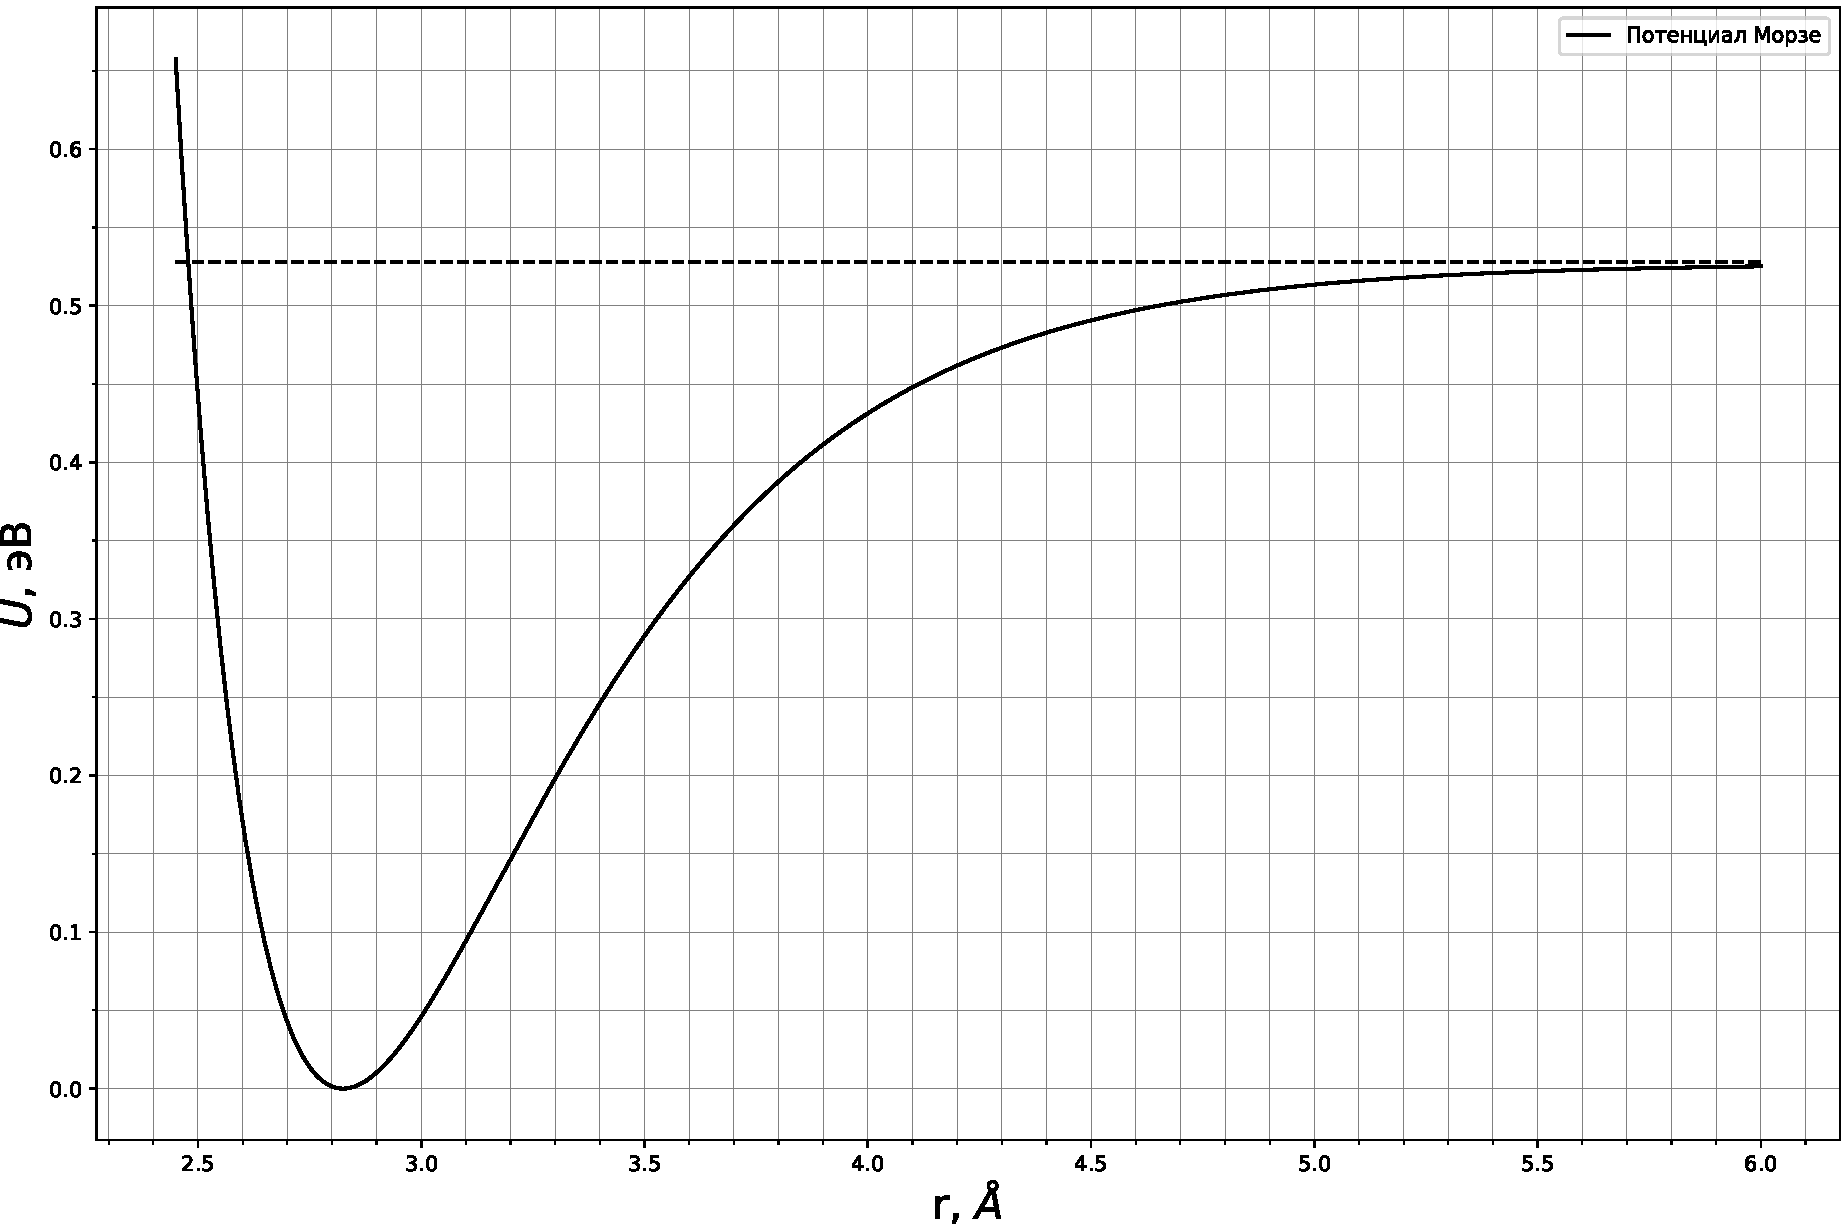
\includegraphics[height=0.45\textheight]{data/morse}
	\caption{Потенциал Морзе для электронного состояния $^3\Pi^+_{0u}$}
	\label{fig:morse}
\end{figure}

\subsection{Результат вычислений}
Все результаты занесем в таблицу \ref{table:final_results}.
% Table generated by Excel2LaTeX from sheet 'Результаты'
\begin{table}[h!]
	\centering
	\caption{Результаты определения молекулярных постоянных}
	\begin{tabular}{|c|c|c|c|c|c|c|}
		\hline
		$T_e$, см$^{-1}$ & $\omega_e'$, см$^{-1}$ & $\omega_e'x_e'$, см$^{-1}$ & $r_e'$, \AA & Энергия диссоциации & $D_0'$, см$^{-1}$; эВ & $D_0''$, см$^{-1}$; эВ \bigstrut\\
		\hline
		\multirow{3}[6]{*}{15774} & \multirow{3}[6]{*}{133} & \multirow{3}[6]{*}{1.06} & \multirow{3}[6]{*}{2.826} & \makecell{По границе \\сплошного спектра} & 4250; 0.528 & 12397; 1.541 \bigstrut\\
		\cline{5-7}       &   &   &   & \makecell{Экстраполяция \\Берджа--Шпонер} & 3776; 0.470 &  \bigstrut\\
		\cline{5-7}       &   &   &   & \makecell{Линейная \\экстраполяция} & 4029; 0.501 &  \bigstrut\\
		\hline
		\multicolumn{7}{|c|}{Табличные данные} \bigstrut\\
		\hline
		15770.6& 125.3  & 0.702  &  3.028 &   & 4320; 0.536  & 12440; 1.542 \bigstrut\\
		\hline
		
	\end{tabular}%
	\label{table:final_results}%
\end{table}%

\subsection{Сравнение спектров при разных ширинах щели}
Проведем сравнение спектров, зарегистрированных при разных ширинах щели (рис. \ref{fig:absorption_spectrum_slit}).
\begin{figure}[H]
	\begin{minipage}[h]{0.5\linewidth}
		\centering
		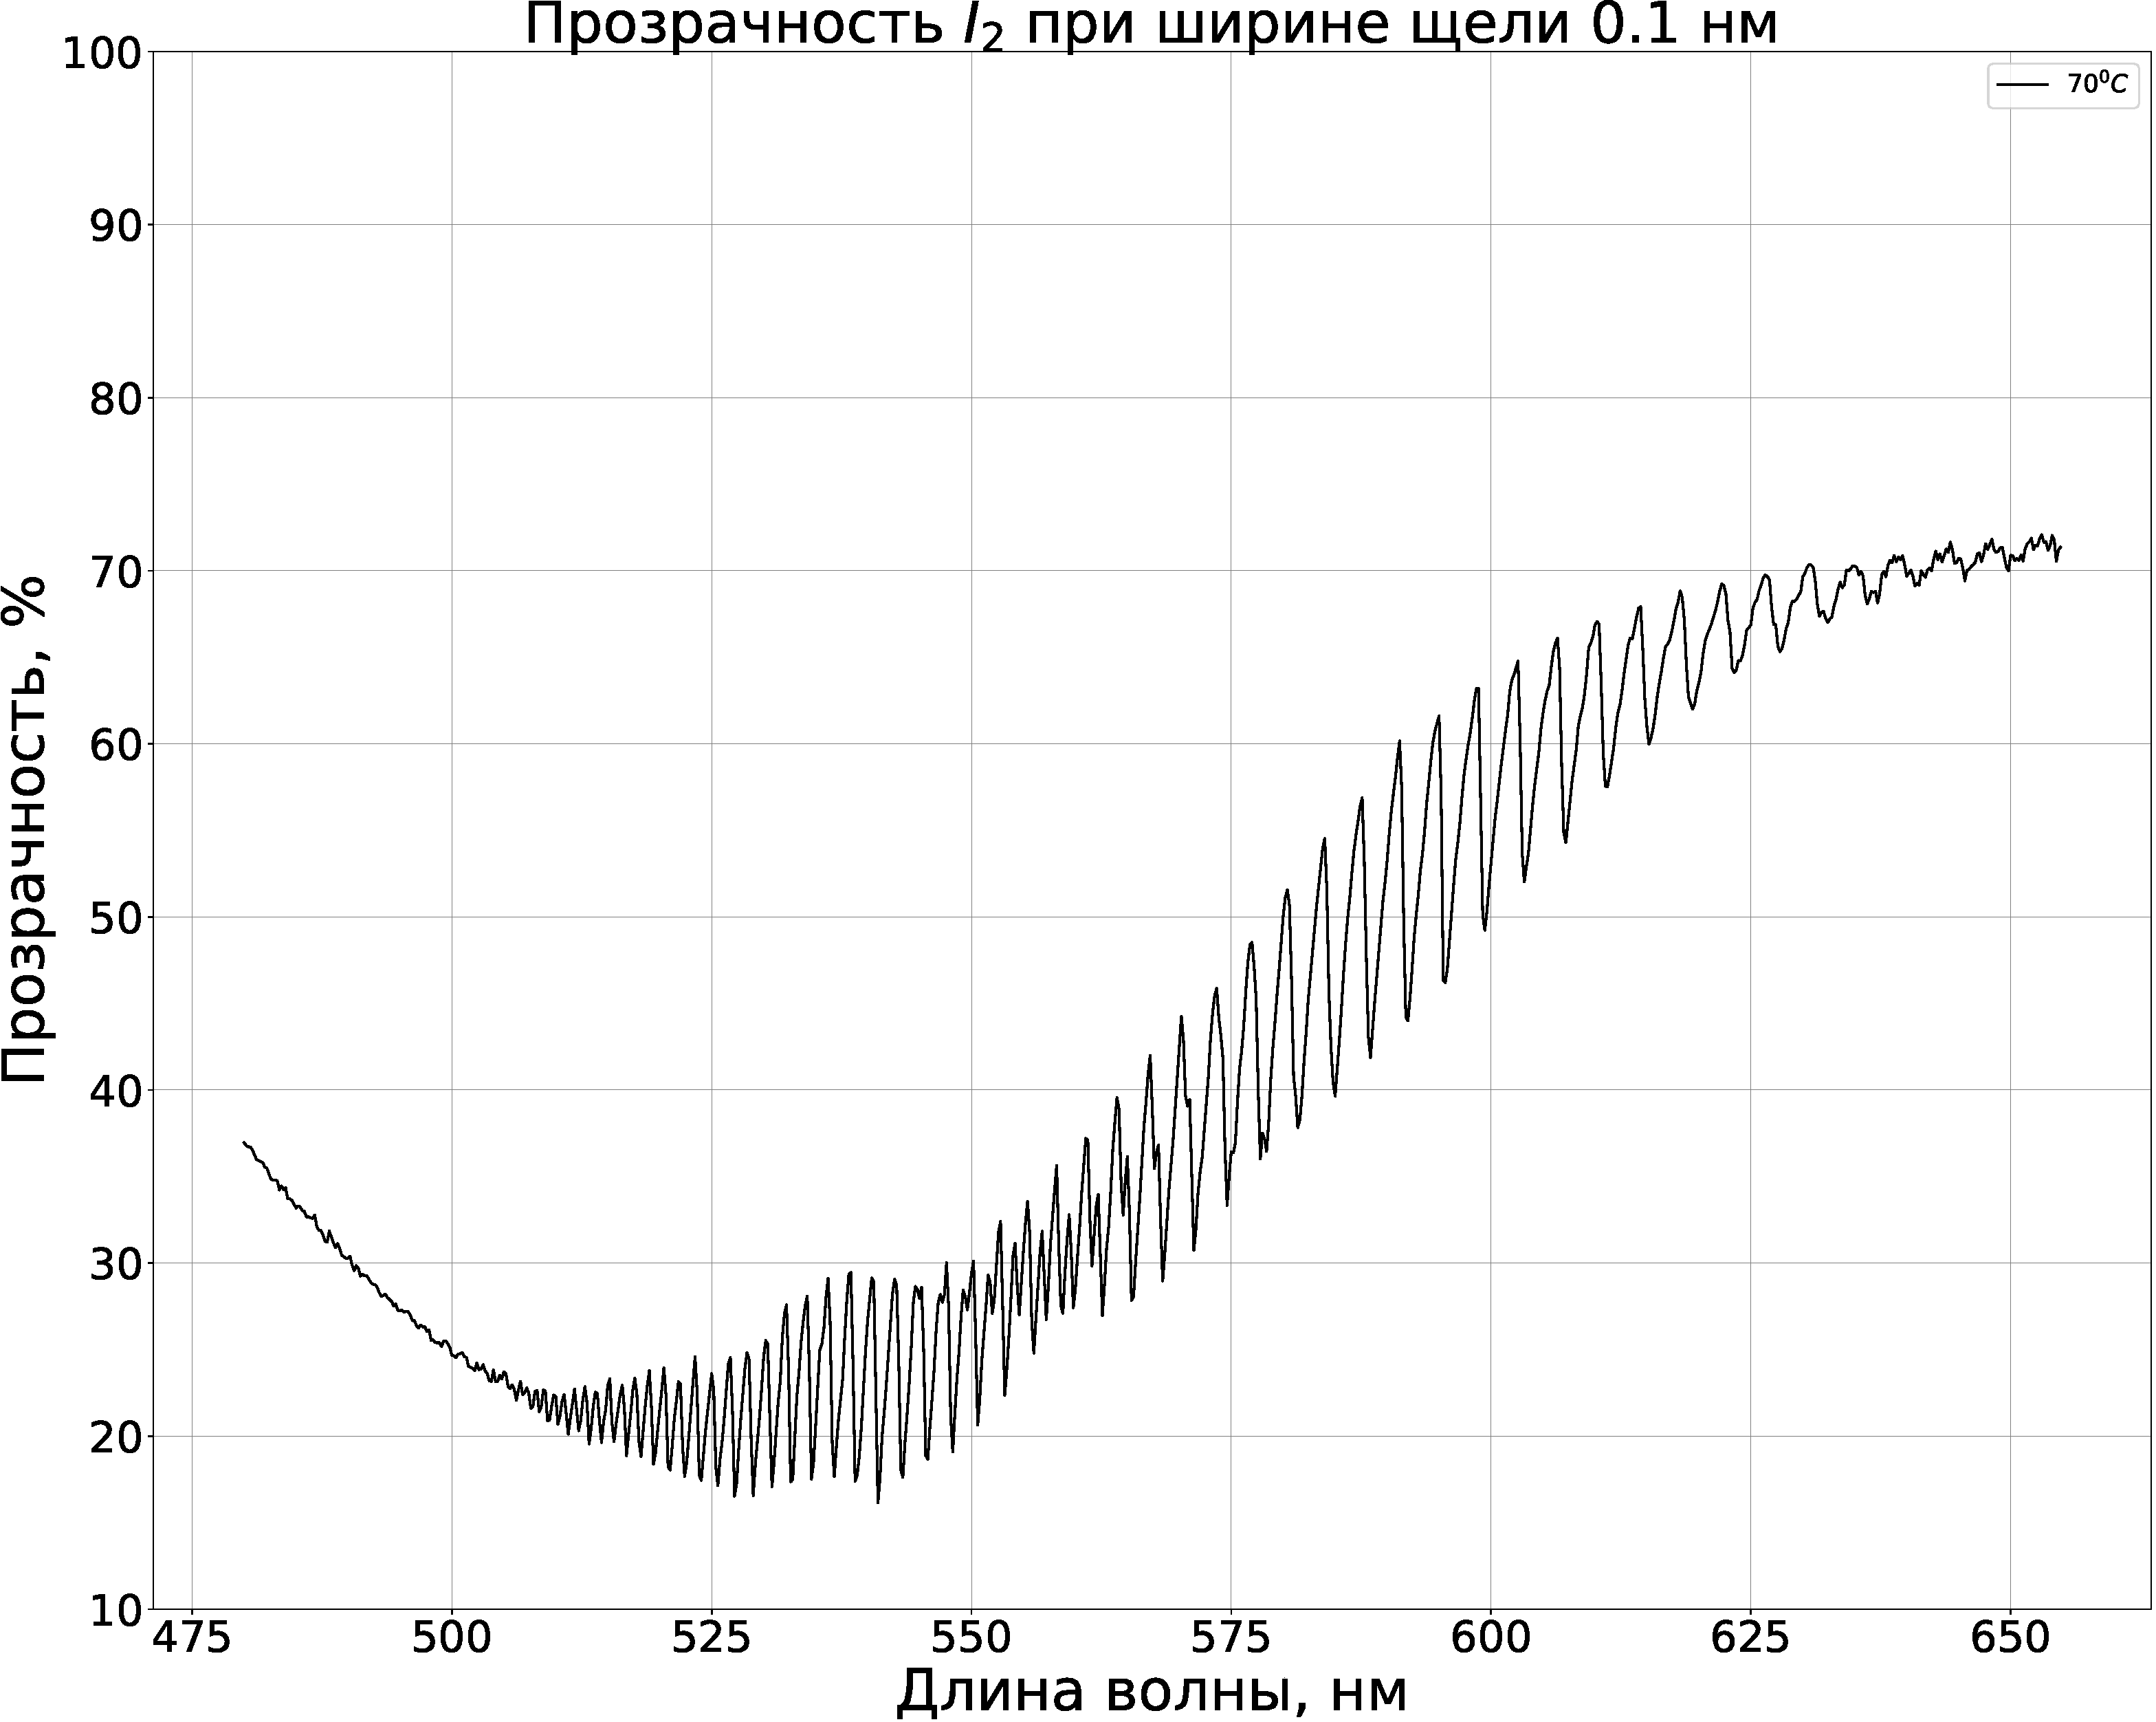
\includegraphics[width=1\linewidth]{data/absorption_spectrum_slit_01}
	\end{minipage}
	\begin{minipage}[h!]{0.5\linewidth}
		\centering
		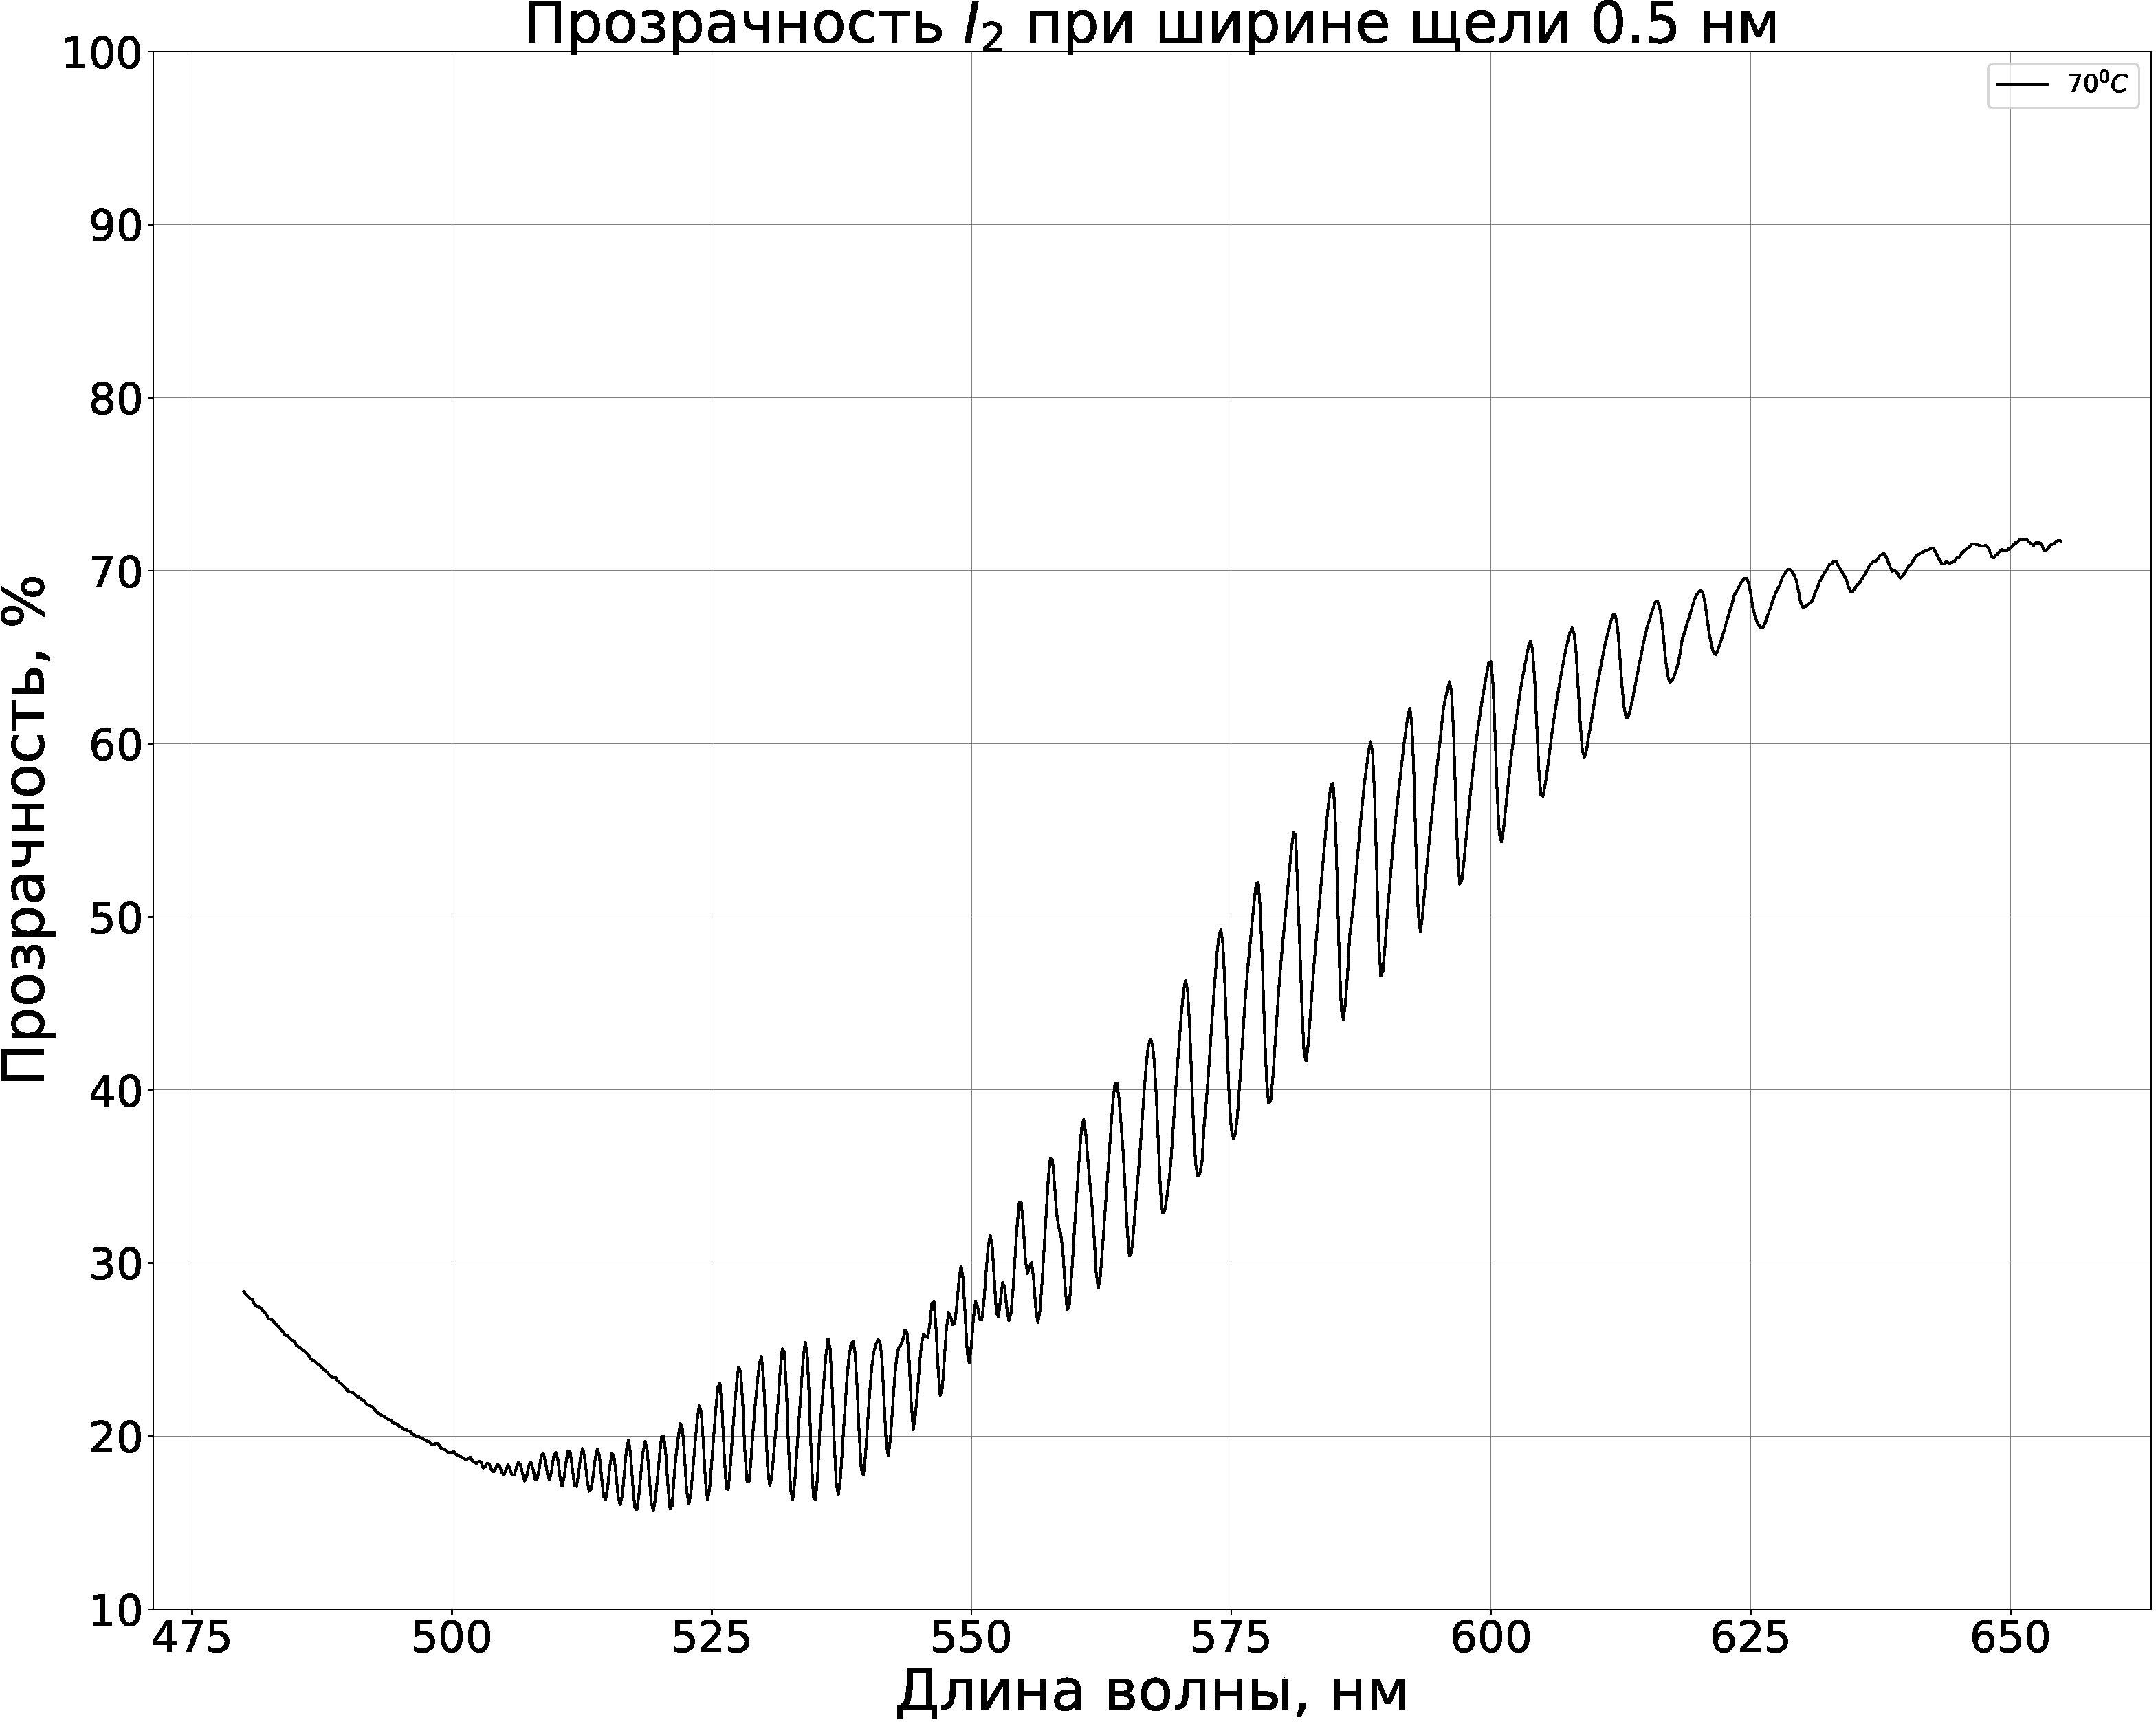
\includegraphics[width=1\linewidth]{data/absorption_spectrum_slit_05}
	\end{minipage}
	\begin{minipage}[h!]{0.5\linewidth}
		\centering
		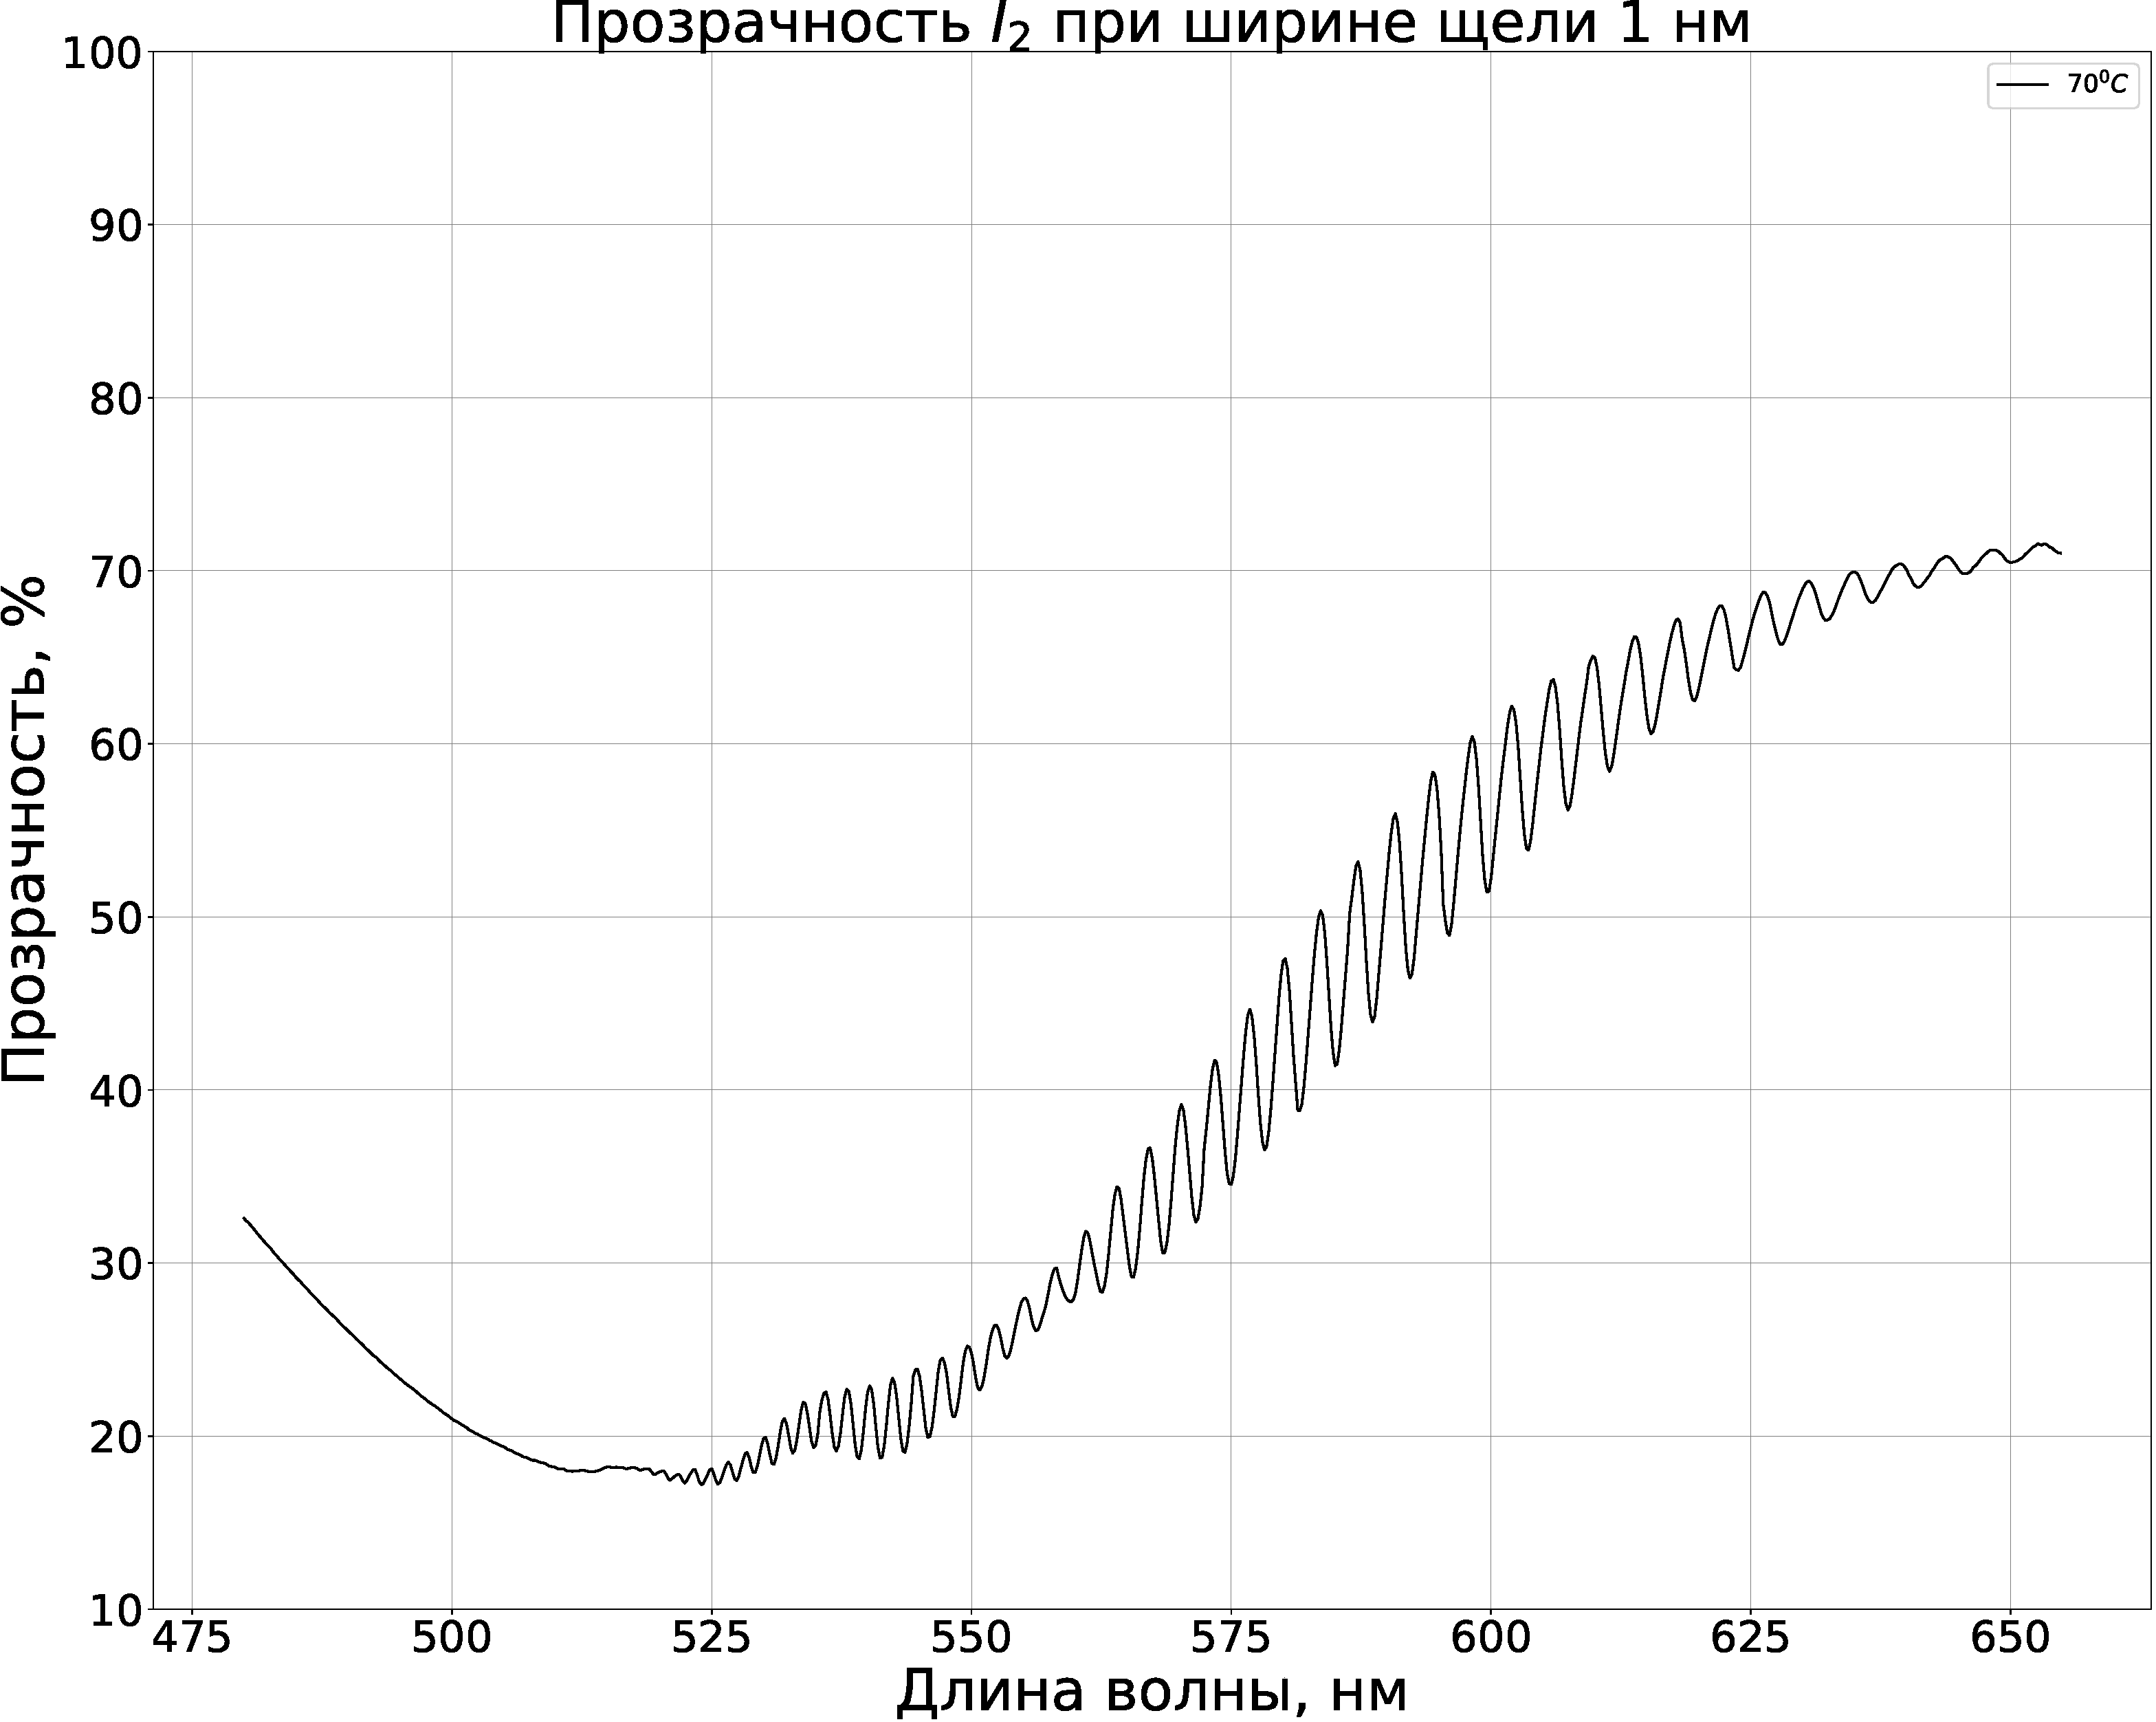
\includegraphics[width=1\linewidth]{data/absorption_spectrum_slit_1}
	\end{minipage}
	\begin{minipage}[h!]{0.5\linewidth}
		\centering
		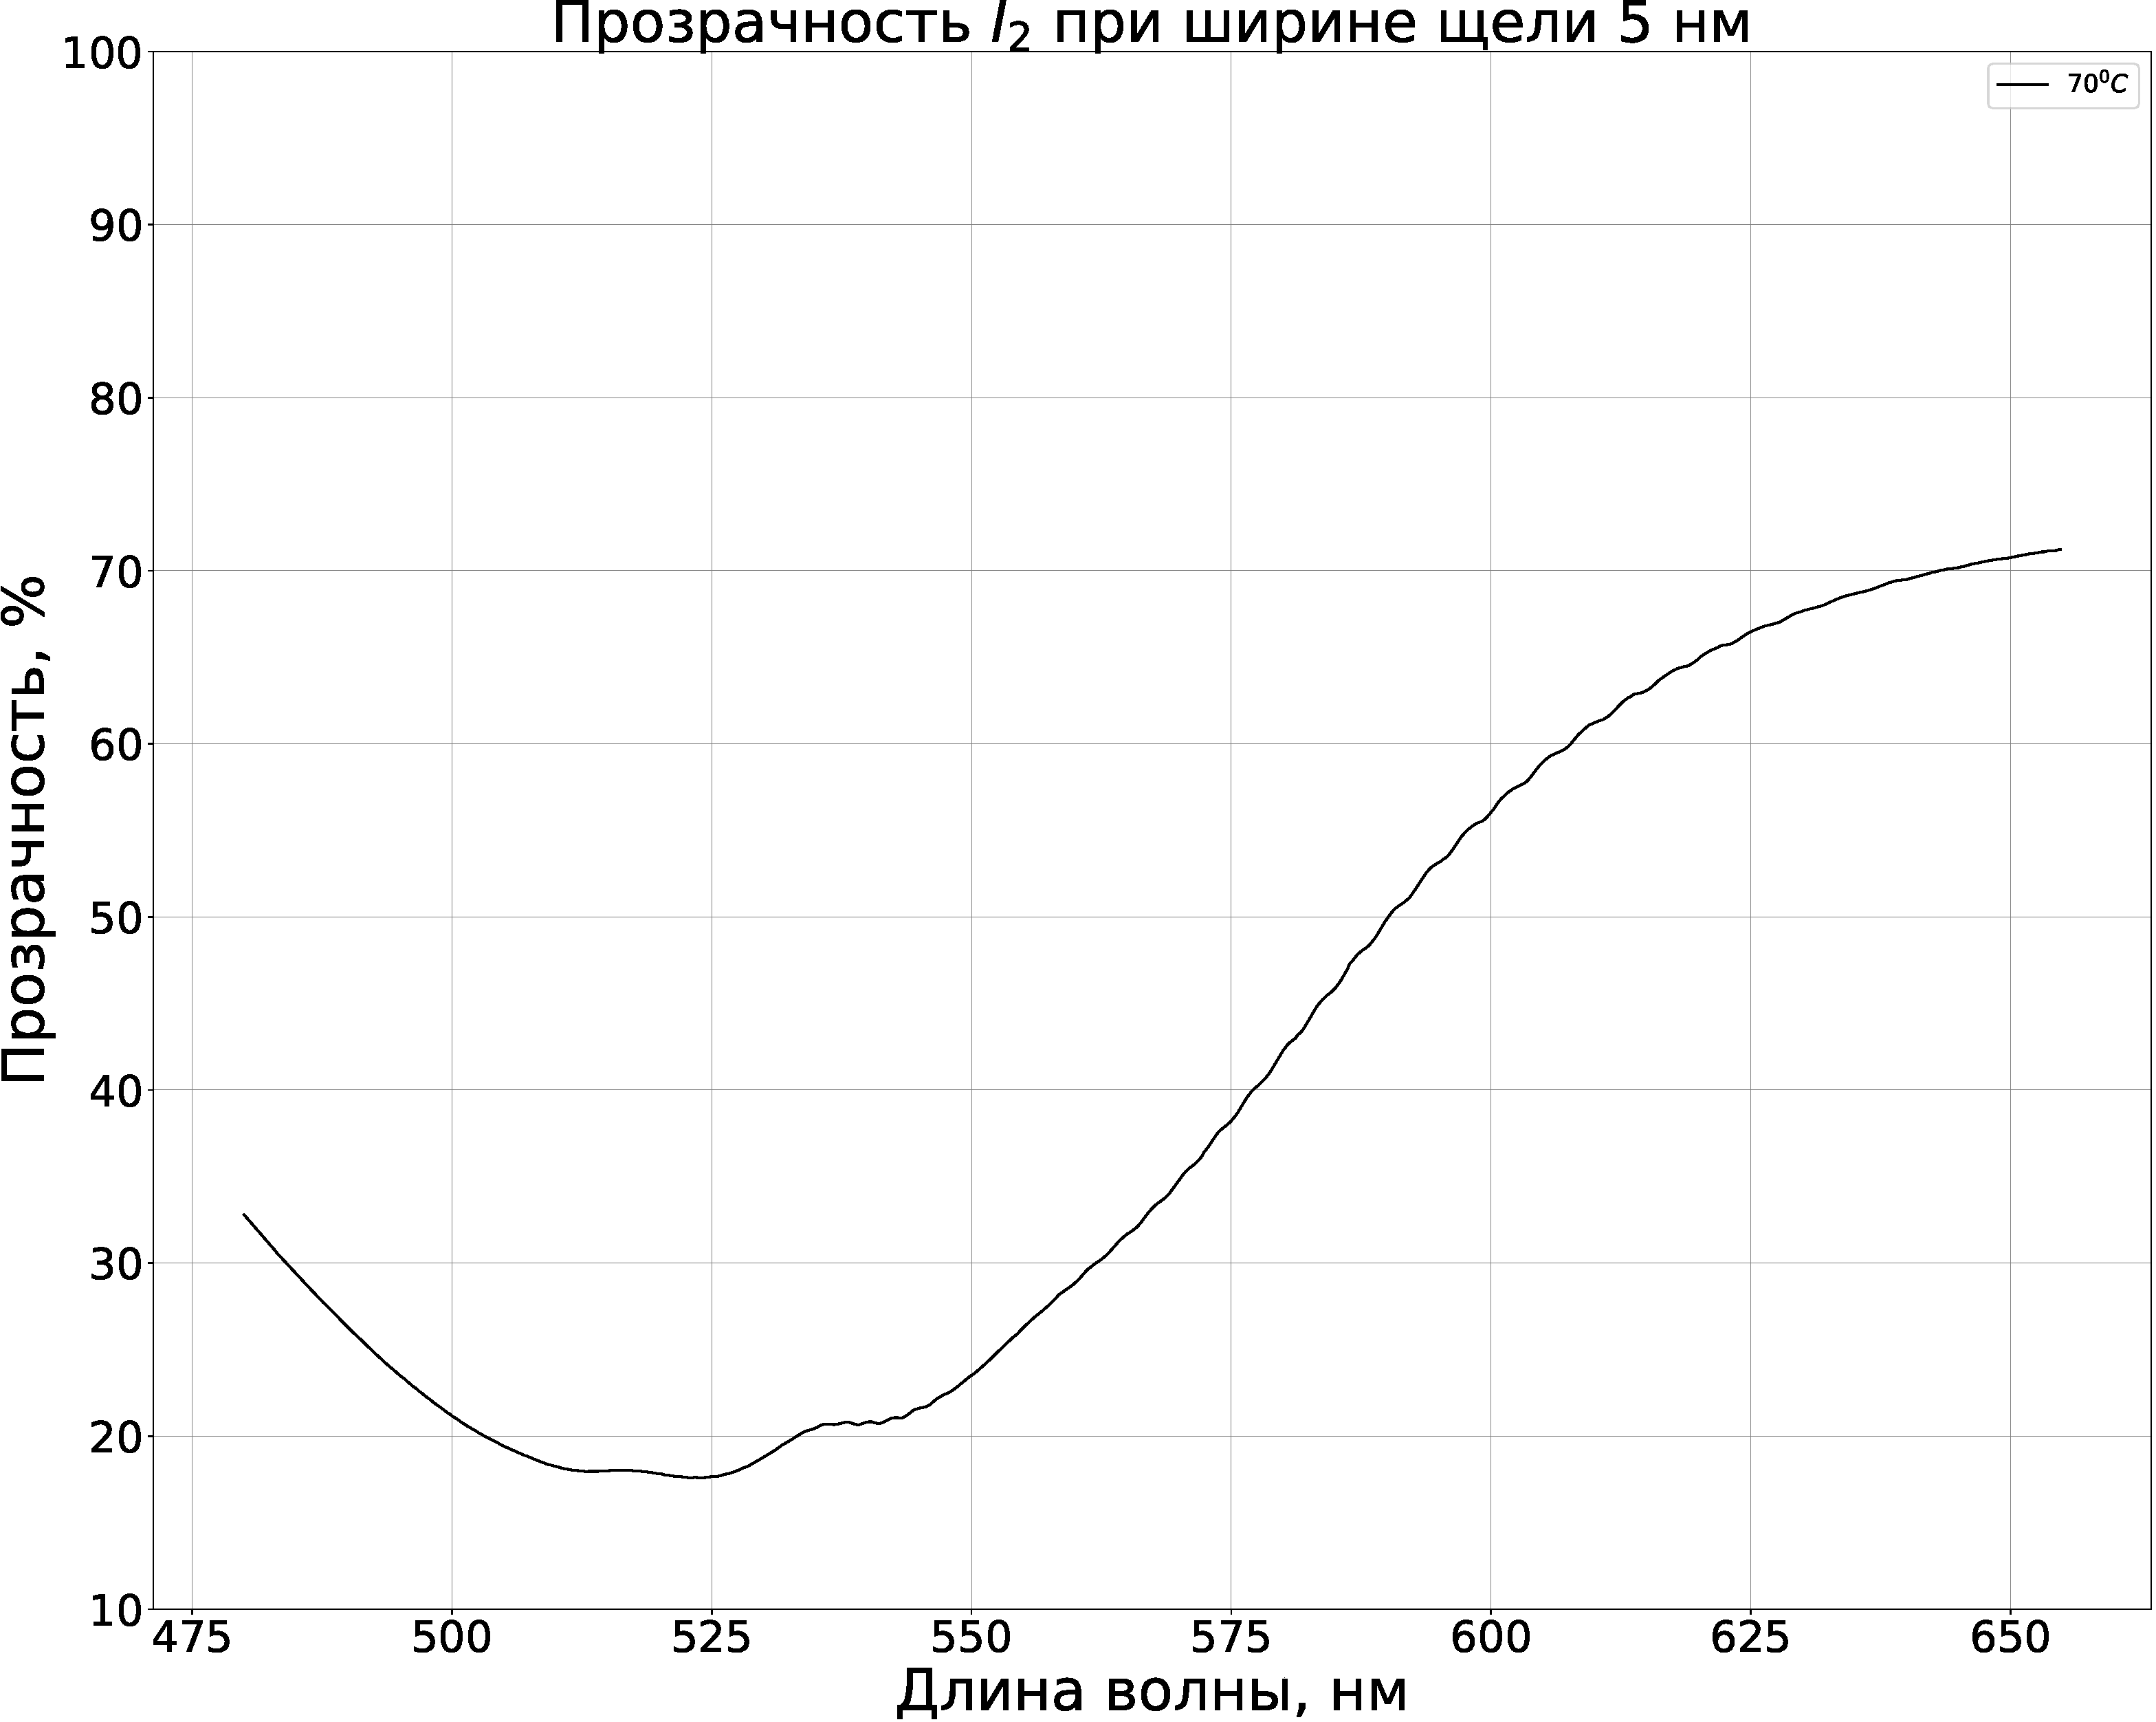
\includegraphics[width=1\linewidth]{data/absorption_spectrum_slit_5}
	\end{minipage}
	\caption{Вид спектра при различных ширинах щели}
	\label{fig:absorption_spectrum_slit}
\end{figure}
Видим, что чем больше размер щели, тем меньшее различие в энергии мы способны различить.





\section{Заключение}
В данной работе рассматривался спектр поглощения молекулы йода. Были получены молекулярные константы, построен потенциал Морзе для возбужденного состояния молекулы $\text{I}_2$.

% TODO: точно у нас так же?
Значения этих констант и названия методов, которыми они были получены приведены в таблице 4.
О соответствии полученных результатов табличным также можно судить из таблицы 4.

Анализ спектров при разных ширинах щели показывает, что с уменьшением размера щели увеличивается разрешающая способность прибора. Электронно-колебательную структуру спектра мы начинаем разрешать при ширине щели около 0.5 нм.



% TODO: проверить библиографию
\begin{thebibliography}{1}
	\bibitem{1}
	С.И. Ткаченко. ИССЛЕДОВАНИЕ ВЕЩЕСТВА ПО ЕГО ИЗЛУЧАТЕЛЬНОПОГЛОЩАТЕЛЬНЫМ ХАРАКТЕРИСТИКАМ.
	МОЛЕКУЛЯРНЫЕ СПЕКТРЫ. Учебно-методическое пособие
	\bibitem{2}
	Справочное издание. — М.: Советская энциклопедия, 1988–1998. — 704 + 704 + 672 + 704 + 760 с.: ил. — ISBN 5-85270-034-7 (т. 1), 5-85270-061-4 (т. 2), 5-85270-019-3 (т. 3), 5-85270-087-8 (т. 4), 5-85270-101-7 (т. 5).
	\bibitem{3}
	Лекции по ФМИ --- Попов Игорь Алексеевич
\end{thebibliography}

%\bibliography{mybibliography}
%\bibliographystyle{gost705}

\end{document}
